% ============================================================
%  Bluetooth Earphone Companion App
%  Low-Fidelity Prototype Report
%  CENG 318 / ID 322 — Spring 2026
% ============================================================
\documentclass[12pt, a4paper]{report}

% ---------- Encoding & Fonts ----------
\usepackage[T1]{fontenc}
\usepackage[utf8]{inputenc}
\usepackage{lmodern}

% ---------- Page Layout ----------
\usepackage[
  top=2.5cm, bottom=2.5cm,
  left=2.5cm, right=2.5cm,
  headheight=14pt
]{geometry}

% ---------- Headers & Footers ----------
\usepackage{fancyhdr}
\pagestyle{fancy}
\fancyhf{}
\fancyhead[L]{\small CENG 318 / ID 322 --- Spring 2026}
\fancyhead[R]{\small Bluetooth Earphone Companion App}
\fancyfoot[C]{\thepage}
\renewcommand{\headrulewidth}{0.4pt}

% ---------- Graphics ----------
\usepackage{graphicx}
\usepackage{float}
\usepackage[labelfont=bf, font=small]{caption}
\usepackage{subcaption}
\graphicspath{{../wireframes/}}

% ---------- Typography ----------
\usepackage{microtype}
\usepackage{parskip}
\usepackage{url}
\setlength{\parindent}{0pt}

% ---------- Tables ----------
\usepackage{booktabs}
\usepackage{tabularx}
\usepackage{longtable}
\usepackage{array}

% ---------- Colours & Boxes ----------
\usepackage{xcolor}

\definecolor{accentblue}{RGB}{30, 100, 200}
\definecolor{lightgray}{RGB}{245, 245, 245}

% Simple highlight box using standard LaTeX (no mdframed)
\newsavebox{\hlbox}
\newenvironment{highlight}{%
  \par\vspace{6pt}%
  \noindent%
  \begin{lrbox}{\hlbox}%
    \begin{minipage}{\dimexpr\linewidth-14pt\relax}%
      \vspace{6pt}\small%
}{%
      \vspace{6pt}%
    \end{minipage}%
  \end{lrbox}%
  \noindent\colorbox{lightgray}{%
    \hspace{2pt}%
    \textcolor{accentblue}{\rule[-0.2\baselineskip]{2pt}{\dimexpr\ht\hlbox+\dp\hlbox\relax}}%
    \hspace{8pt}\usebox{\hlbox}\hspace{2pt}%
  }%
  \par\vspace{6pt}%
}

% ---------- Lists ----------
\usepackage{enumitem}
\setlist[itemize]{topsep=4pt, itemsep=2pt}

% ---------- Hyperlinks ----------
\usepackage[
  colorlinks=true,
  linkcolor=accentblue,
  urlcolor=accentblue,
  citecolor=accentblue,
  bookmarks=true,
  pdfauthor={CENG318/ID322 Team},
  pdftitle={Bluetooth Earphone Companion App --- Low-Fidelity Prototype Report}
]{hyperref}

% ============================================================
\begin{document}
% ============================================================

% ---- Title page ----
\begin{titlepage}
  \centering
  \vspace*{2cm}
  {\large\bfseries CENG 318 / ID 322 --- Spring 2026}\par
  \vspace{1cm}
  \rule{\linewidth}{1.5pt}\par\vspace{0.5cm}
  {\Huge\bfseries Bluetooth Earphone\\[0.3cm]Companion App}\par
  \vspace{0.4cm}
  {\LARGE Low-Fidelity Prototype Report}\par
  \vspace{0.5cm}
  \rule{\linewidth}{1.5pt}\par
  \vspace{1.5cm}

  {\large
    \begin{tabular}{ll}
      \toprule
      \textbf{Name} & \textbf{Role} \\
      \midrule
      Member 1 & Team Coordinator \\
      Member 2 & UX Flow \& Wireframe Lead \\
      Member 3 & Prototype \& Mockup Lead \\
      Member 4 & Report \& Presentation Lead \\
      \bottomrule
    \end{tabular}
  }\par
  \vspace{1.5cm}

  \begin{highlight}
    \textbf{Assignment:} Design a low-fidelity prototype of a digital user interface
    for a Bluetooth earphone companion application on smartphones/tablets, exploring
    interaction flows, layout, and user experience principles.
  \end{highlight}

  \vfill
  {\large April 2026}
\end{titlepage}

% ---- Front matter ----
\tableofcontents
\clearpage

% ============================================================
\chapter{Project Overview \& Objectives}
% ============================================================

\section{Assignment Context}

This report documents the collaborative low-fidelity (lo-fi) prototype design
process for the joint \textbf{CENG 318 / ID 322} course project (Spring 2026). The
project combines industrial design with computer engineering to produce a digital
companion application for a Bluetooth earphone product.

\begin{highlight}
  \textbf{Low-fidelity prototyping} focuses on structure and flow rather than
  visual polish. Materials are simple --- paper sketches, pencil drawings, or
  quick digital drafts --- and iteration is fast, so ideas can be tested and
  changed at low cost before any implementation effort is committed.
\end{highlight}

\section{Project Objectives}

\begin{itemize}
  \item Develop a low-fidelity prototype of a Bluetooth earphone companion app UI
    for smartphones/tablets.
  \item Explore how users interact with the product's core functions.
  \item Emphasise usability, accessibility, and user experience principles.
  \item Document all design versions in order and justify changes between them.
\end{itemize}

\section{Product Vision}

The app allows users to \textbf{connect, monitor, and personalise} their Bluetooth
earphones from a mobile device. Core everyday tasks it supports:

\begin{itemize}
  \item Pair earphones quickly and see connection status at a glance.
  \item Check battery level without picking up the earphones.
  \item Adjust sound with one-tap presets or manual Bass/Mid/Treble sliders.
  \item Switch listening mode (Noise Cancellation / Normal / Transparency) in
    one tap.
  \item Manage account and device settings without navigating deep menus.
\end{itemize}

% ============================================================
\chapter{App Flow \& Navigation Structure}
% ============================================================

\section{Navigation Evolution Summary}

The bottom navigation bar changed across the two prototype versions:

\begin{center}
  \begin{tabular}{p{3cm} p{5cm} p{5.5cm}}
    \toprule
    \textbf{Version} & \textbf{Bottom Nav Tabs} & \textbf{Key Change} \\
    \midrule
    Version 1 & Devices \textbar{} Profile
      & Two tabs; all controls via gear icon \\
    Version 2 & Home \textbar{} Sound \textbar{} Noise \textbar{} Profile
      & Four tabs; audio controls surfaced directly \\
    \bottomrule
  \end{tabular}
\end{center}

\section{Screen Inventory}

The table below lists every wireframe asset with its version, location, and role.
Paths are relative to \texttt{docs/wireframes/}.

% Use \small + url-style path to avoid overflowing columns
\begin{center}
\small
\begin{longtable}{p{1.5cm} p{5.8cm} p{5.5cm}}
  \toprule
  \textbf{Ver.} & \textbf{File path} & \textbf{Role in flow} \\
  \midrule
  \endhead
  v1 & \path{devices/wireframe-devices-home-empty.jpeg}
     & Home empty state, Add Device CTA \\[2pt]
  v1 & \path{devices/wireframe-devices-list-populated.jpeg}
     & Home with a paired device card \\[2pt]
  v1 & \path{devices/wireframe-device-control-equalizer.jpeg}
     & Per-device: model, battery, modes, EQ \\[2pt]
  v1 & \path{profile/wireframe-login.jpeg}
     & Login entry from Profile tab \\[2pt]
  v1 & \path{profile/wireframe-register.jpeg}
     & New account creation \\[2pt]
  v1 & \path{profile/wireframe-profile-overview.jpeg}
     & After-login account summary \\[2pt]
  v1 & \path{profile/wireframe-profile-menu.jpeg}
     & After-login menu list layout \\[2pt]
  v1 & \path{profile/wireframe-forgot-password-and-login.jpeg}
     & Forgot password + login composite \\[2pt]
  v1 & \path{settings/wireframe-settings-general.jpeg}
     & Language, theme, device settings entry \\[2pt]
  v1 & \path{settings/wireframe-settings-device-detail.jpeg}
     & Device image, serial, power-off, updates \\[2pt]
  v1 & \path{settings/wireframe-settings-automatic-power-off.jpeg}
     & Auto power-off duration picker \\[2pt]
  v1 & \path{flowsheets/flowsheet-add-device-and-settings.jpeg}
     & Flow: empty home $\to$ BT $\to$ list $\to$ settings \\[2pt]
  v1 & \path{flowsheets/flowsheet-auth-and-profile.jpeg}
     & Flow: login $\to$ register $\to$ profile $\to$ forgot pw \\[2pt]
  v1 & \path{flowsheets/flowsheet-bluetooth-pairing.jpeg}
     & BT searching $\to$ My Devices transition \\[2pt]
  v1 & \path{flowsheets/flowsheet-device-settings-and-power-off.jpeg}
     & Device detail $\to$ auto power-off \\[6pt]
  v2 & \path{hand-drawn/wireframe-sound-equalizer-presets-sliders.jpeg}
     & Sound tab: presets, sliders, Save \\[2pt]
  v2 & \path{hand-drawn/wireframe-volume-overlay-vertical.jpeg}
     & Volume capsule overlay (ephemeral) \\[2pt]
  v2 & \path{figma-v3/wireframe-sound-equalizer-four-presets.jpeg}
     & Figma Sound: four presets + Custom \\[2pt]
  v2 & \path{figma-v3/wireframe-sound-equalizer-custom-save.jpeg}
     & Figma Sound: presets + sliders + Save \\[2pt]
  v2 & \path{flowsheets/flowsheet-nine-screen-home-volume-settings-profile.jpeg}
     & Nine-panel: splash $\to$ pair $\to$ home $\to$ tabs \\[2pt]
  v2 & \path{flowsheets/flowsheet-statistics-history-mydevices-bud-controls.jpeg}
     & Five-panel: stats, history, devices, buds \\
  \bottomrule
  \caption{Complete wireframe asset inventory}
\end{longtable}
\end{center}

% ============================================================
\chapter{Version 1 --- Paper Wireframe Prototypes}
% ============================================================

\section{Overview}

Version 1 consists of hand-drawn wireframes on paper, photographed to create the
design record. At this stage the navigation chrome used \textbf{two bottom tabs}:
\textbf{Devices} and \textbf{Profile}. Settings were accessed via a gear icon in
the header rather than a dedicated tab. Screens were designed screen-by-screen and
then combined into multi-screen flowsheets to verify the transitions.

% -------------------------------------------------------
\section{Home / Device Screens}
% -------------------------------------------------------

\subsection{Empty Home State}

\begin{figure}[H]
  \centering
  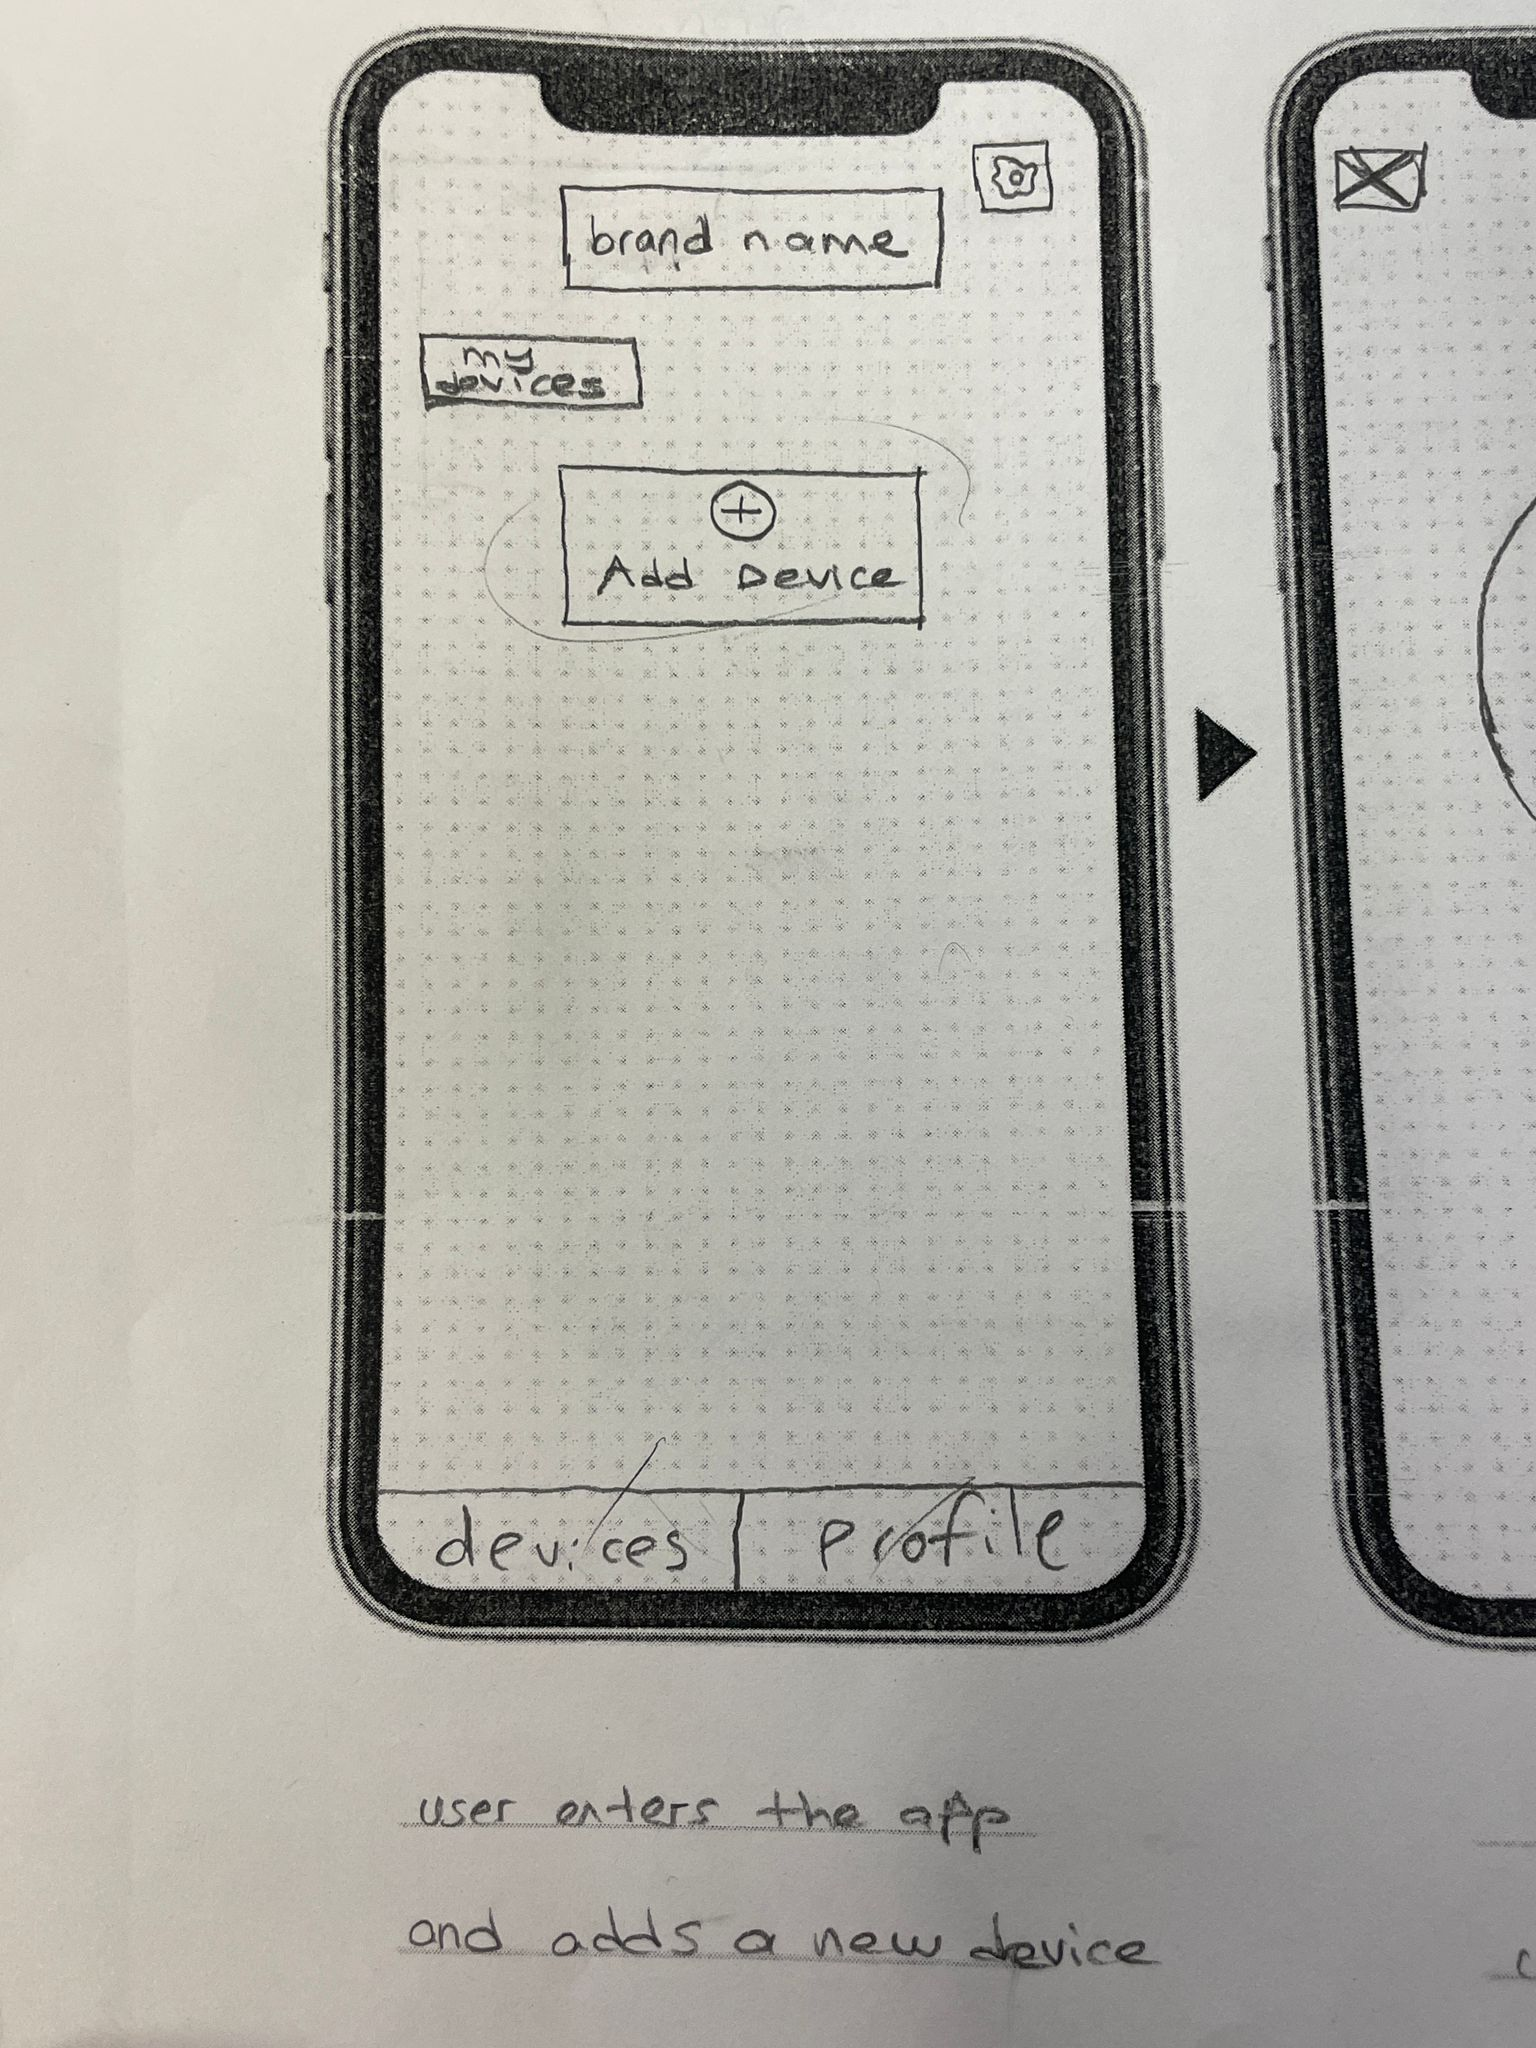
\includegraphics[width=0.42\textwidth]{devices/wireframe-devices-home-empty.jpeg}
  \caption{Home --- empty state. ``My Devices'' section is empty; the large
    \textbf{Add Device (+)} button is the only call-to-action, guiding first-time
    users without ambiguity.}
  \label{fig:v1-home-empty}
\end{figure}

\subsection{Populated Home State}

\begin{figure}[H]
  \centering
  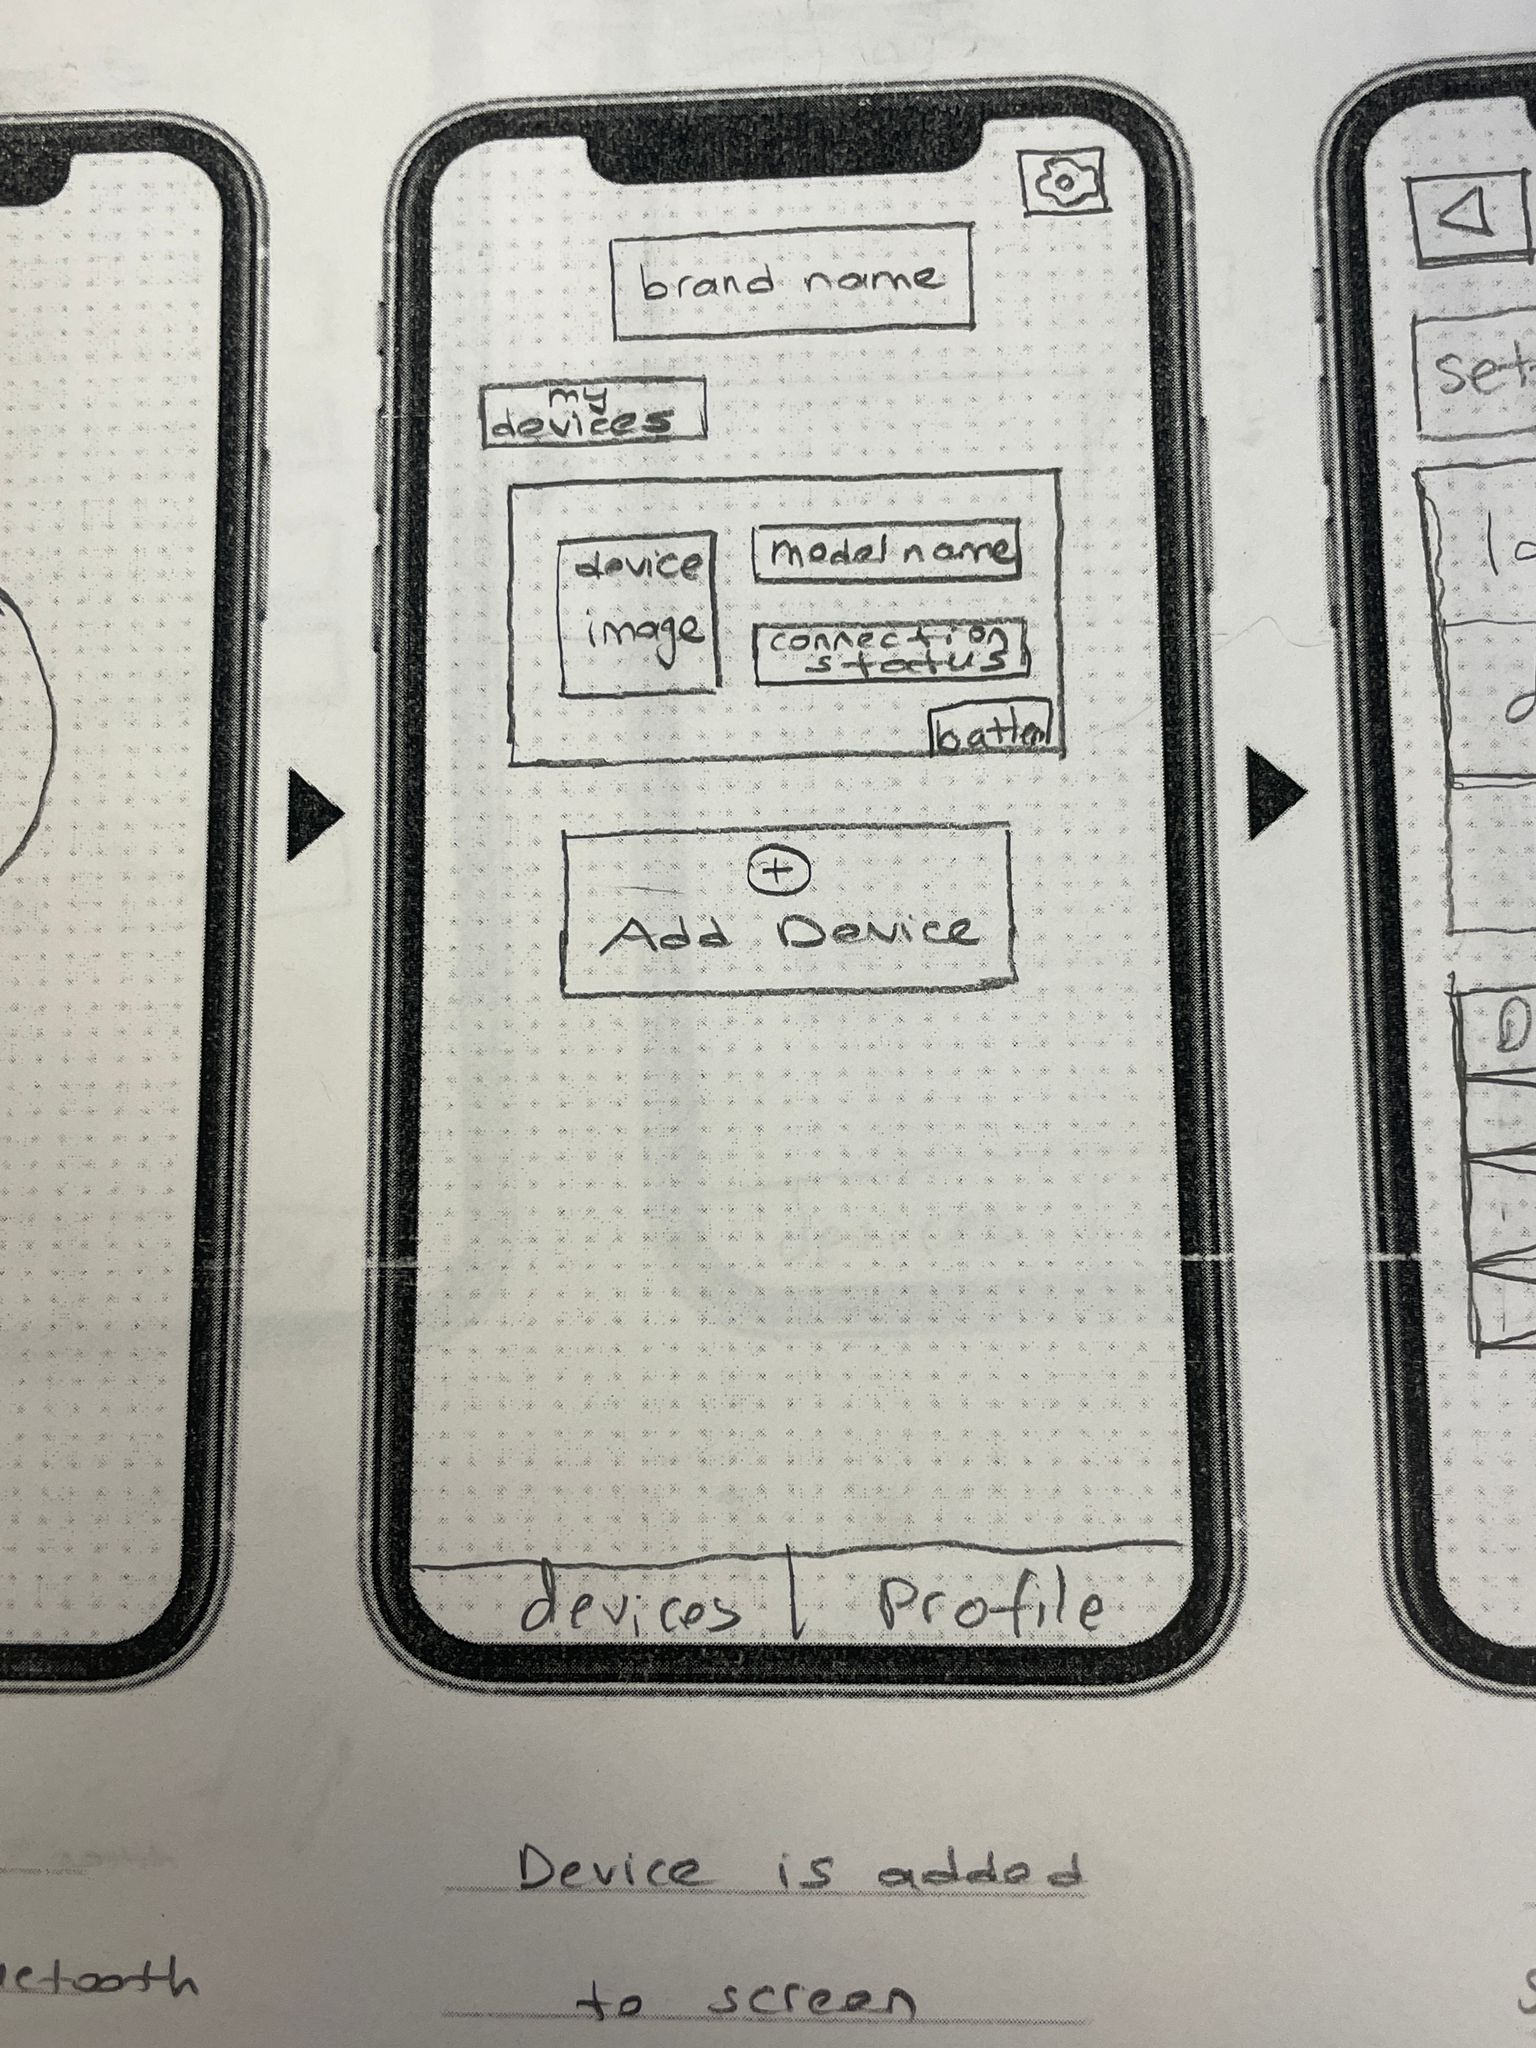
\includegraphics[width=0.42\textwidth]{devices/wireframe-devices-list-populated.jpeg}
  \caption{Home --- populated state. A device card shows model image, name,
    connection status, and battery. Add Device remains visible for
    multi-device management.}
  \label{fig:v1-home-populated}
\end{figure}

\subsection{Device Control \& Equalizer}

\begin{figure}[H]
  \centering
  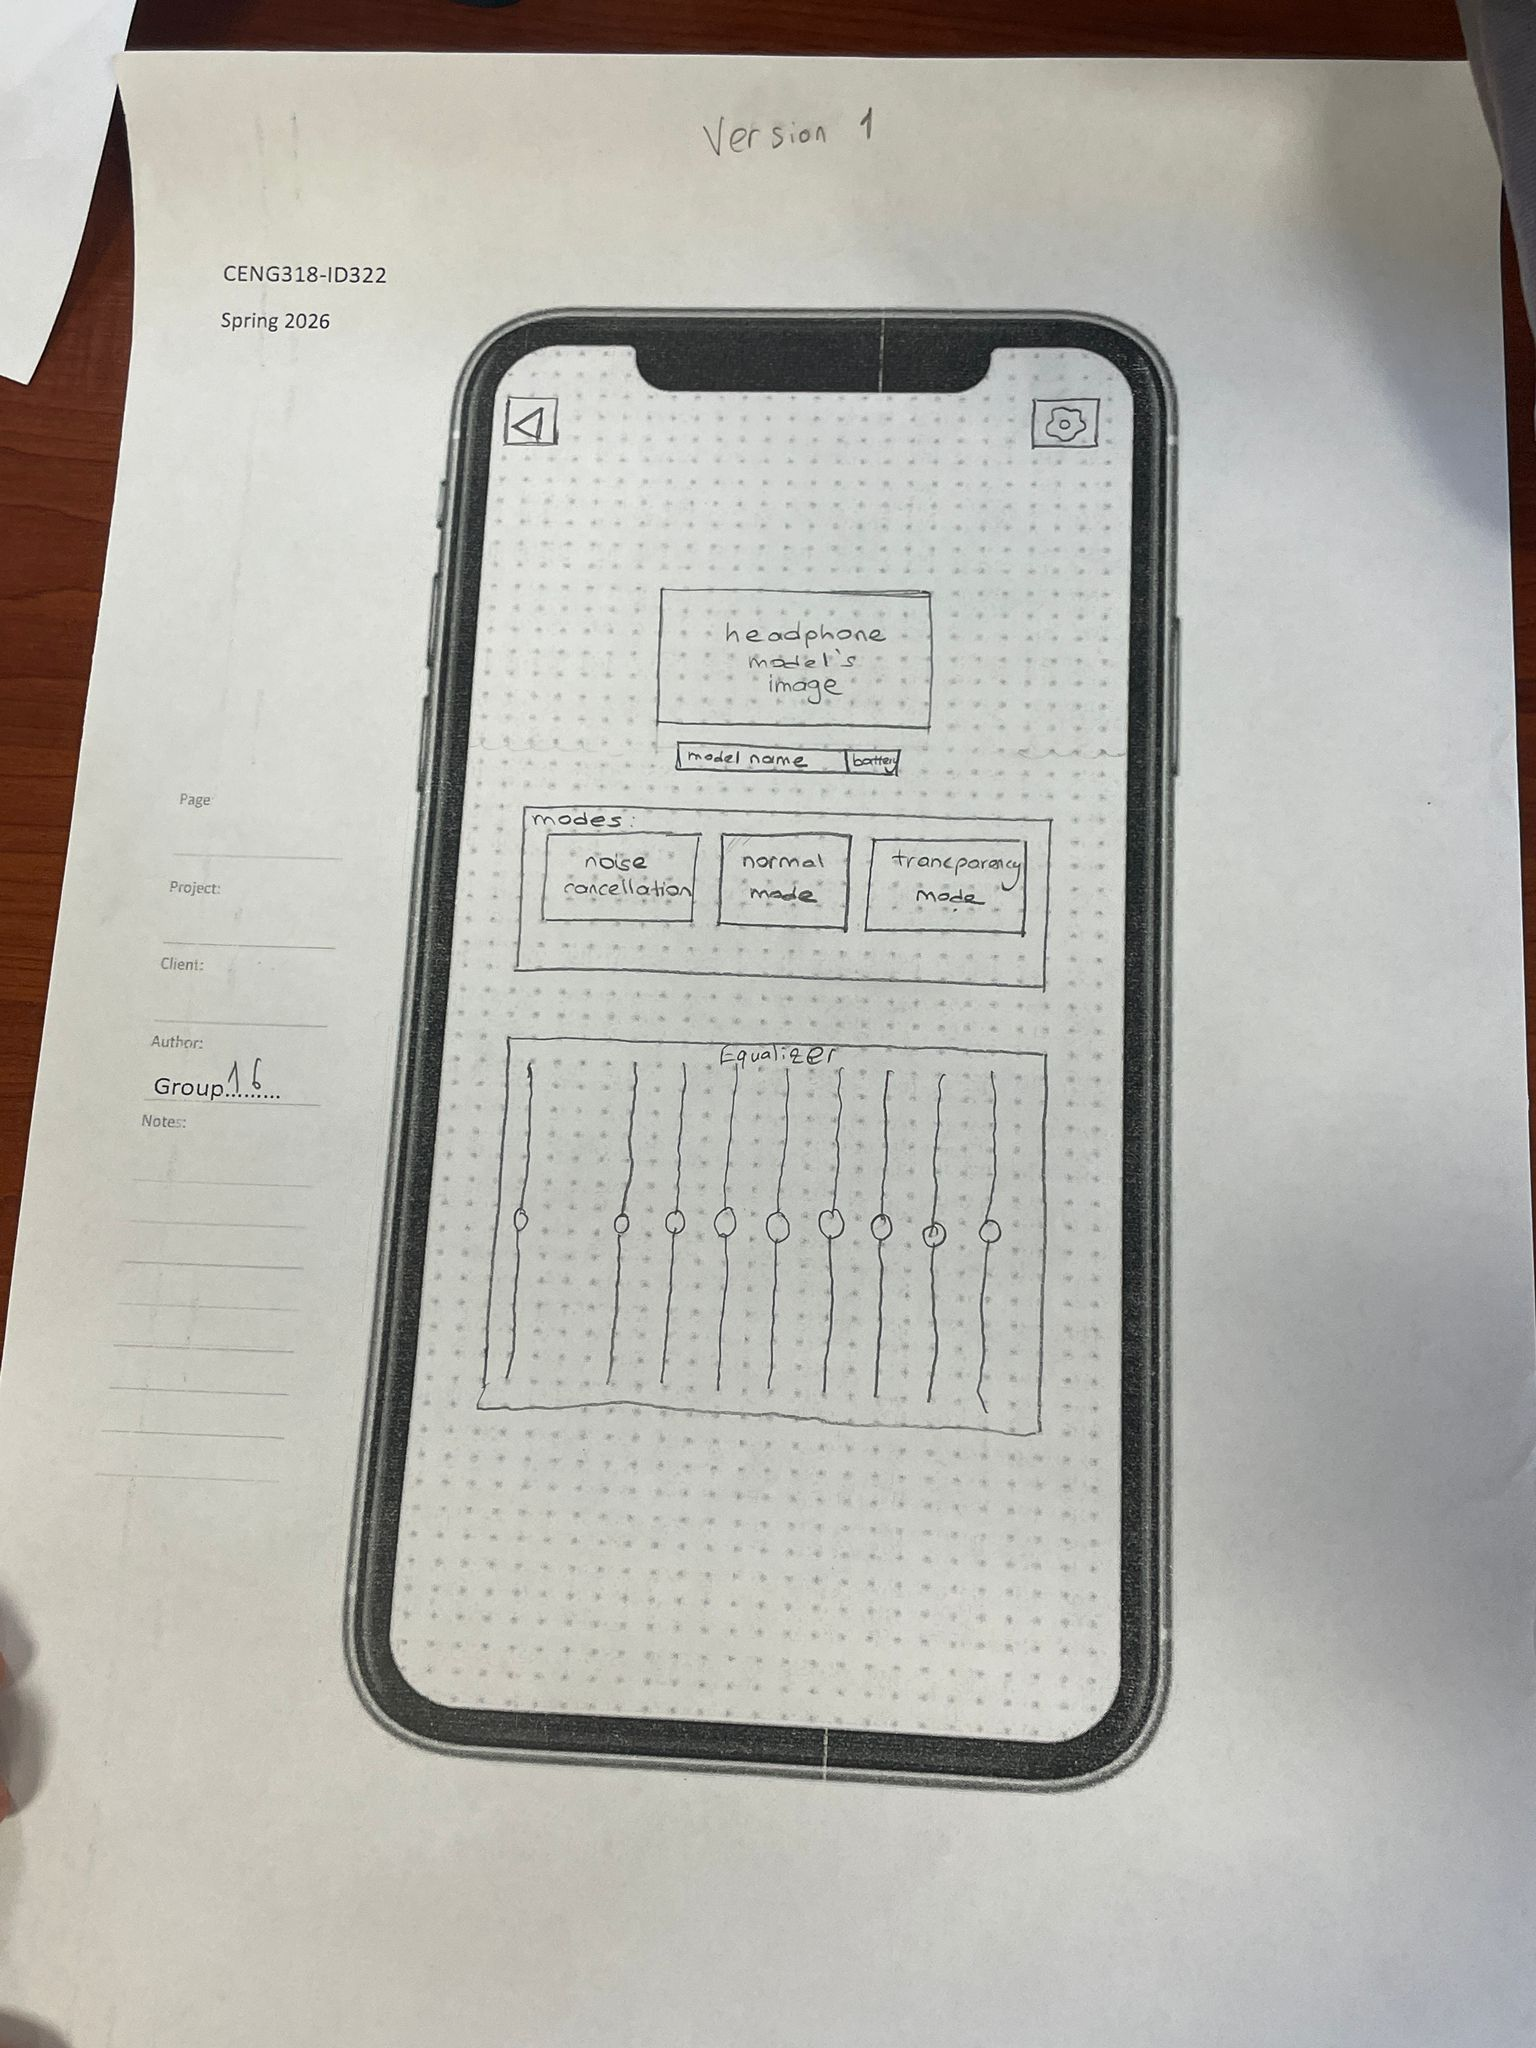
\includegraphics[width=0.42\textwidth]{devices/wireframe-device-control-equalizer.jpeg}
  \caption{Device control screen (Version 1). One combined surface shows the
    headphone image, model/battery, three listening mode buttons, and a
    multi-band vertical equalizer.}
  \label{fig:v1-device-eq}
\end{figure}

This combined control surface (Figure~\ref{fig:v1-device-eq}) was the first attempt
at grouping all device actions together. After review, this approach was considered
too dense and was split into dedicated tabs in Version~2.

% -------------------------------------------------------
\section{Profile \& Authentication Screens}
% -------------------------------------------------------

\subsection{Login}

\begin{figure}[H]
  \centering
  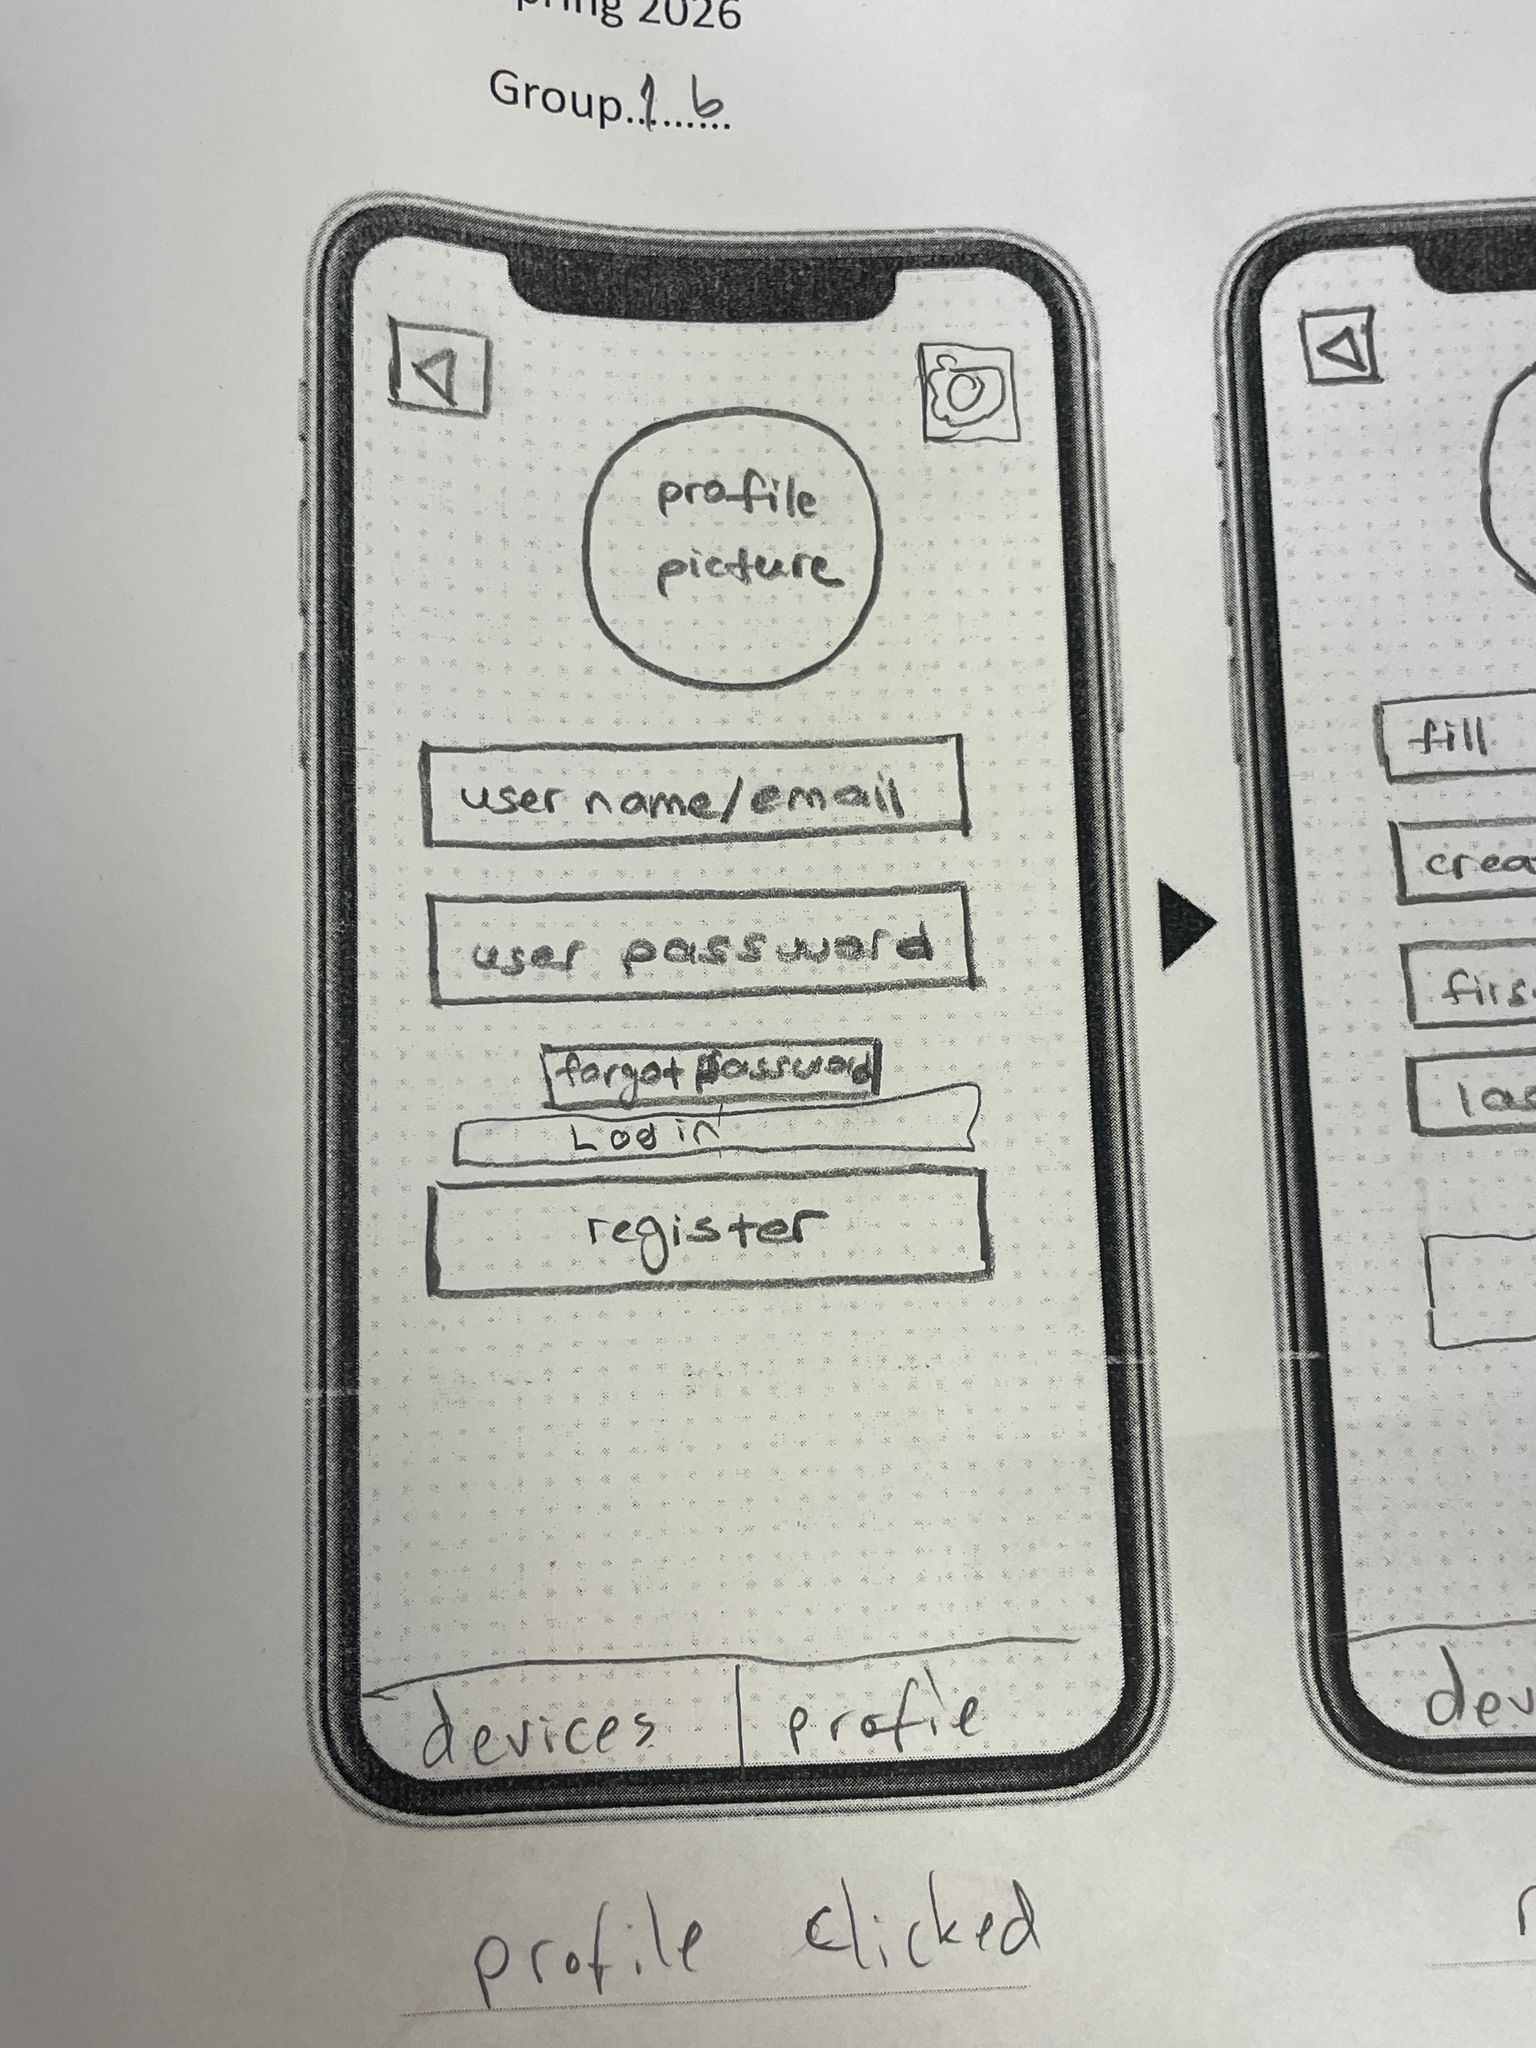
\includegraphics[width=0.42\textwidth]{profile/wireframe-login.jpeg}
  \caption{Login screen --- accessed by tapping the Profile tab.
    Fields: username/email and password. Links: Forgot Password and Register.}
  \label{fig:v1-login}
\end{figure}

\subsection{Register}

\begin{figure}[H]
  \centering
  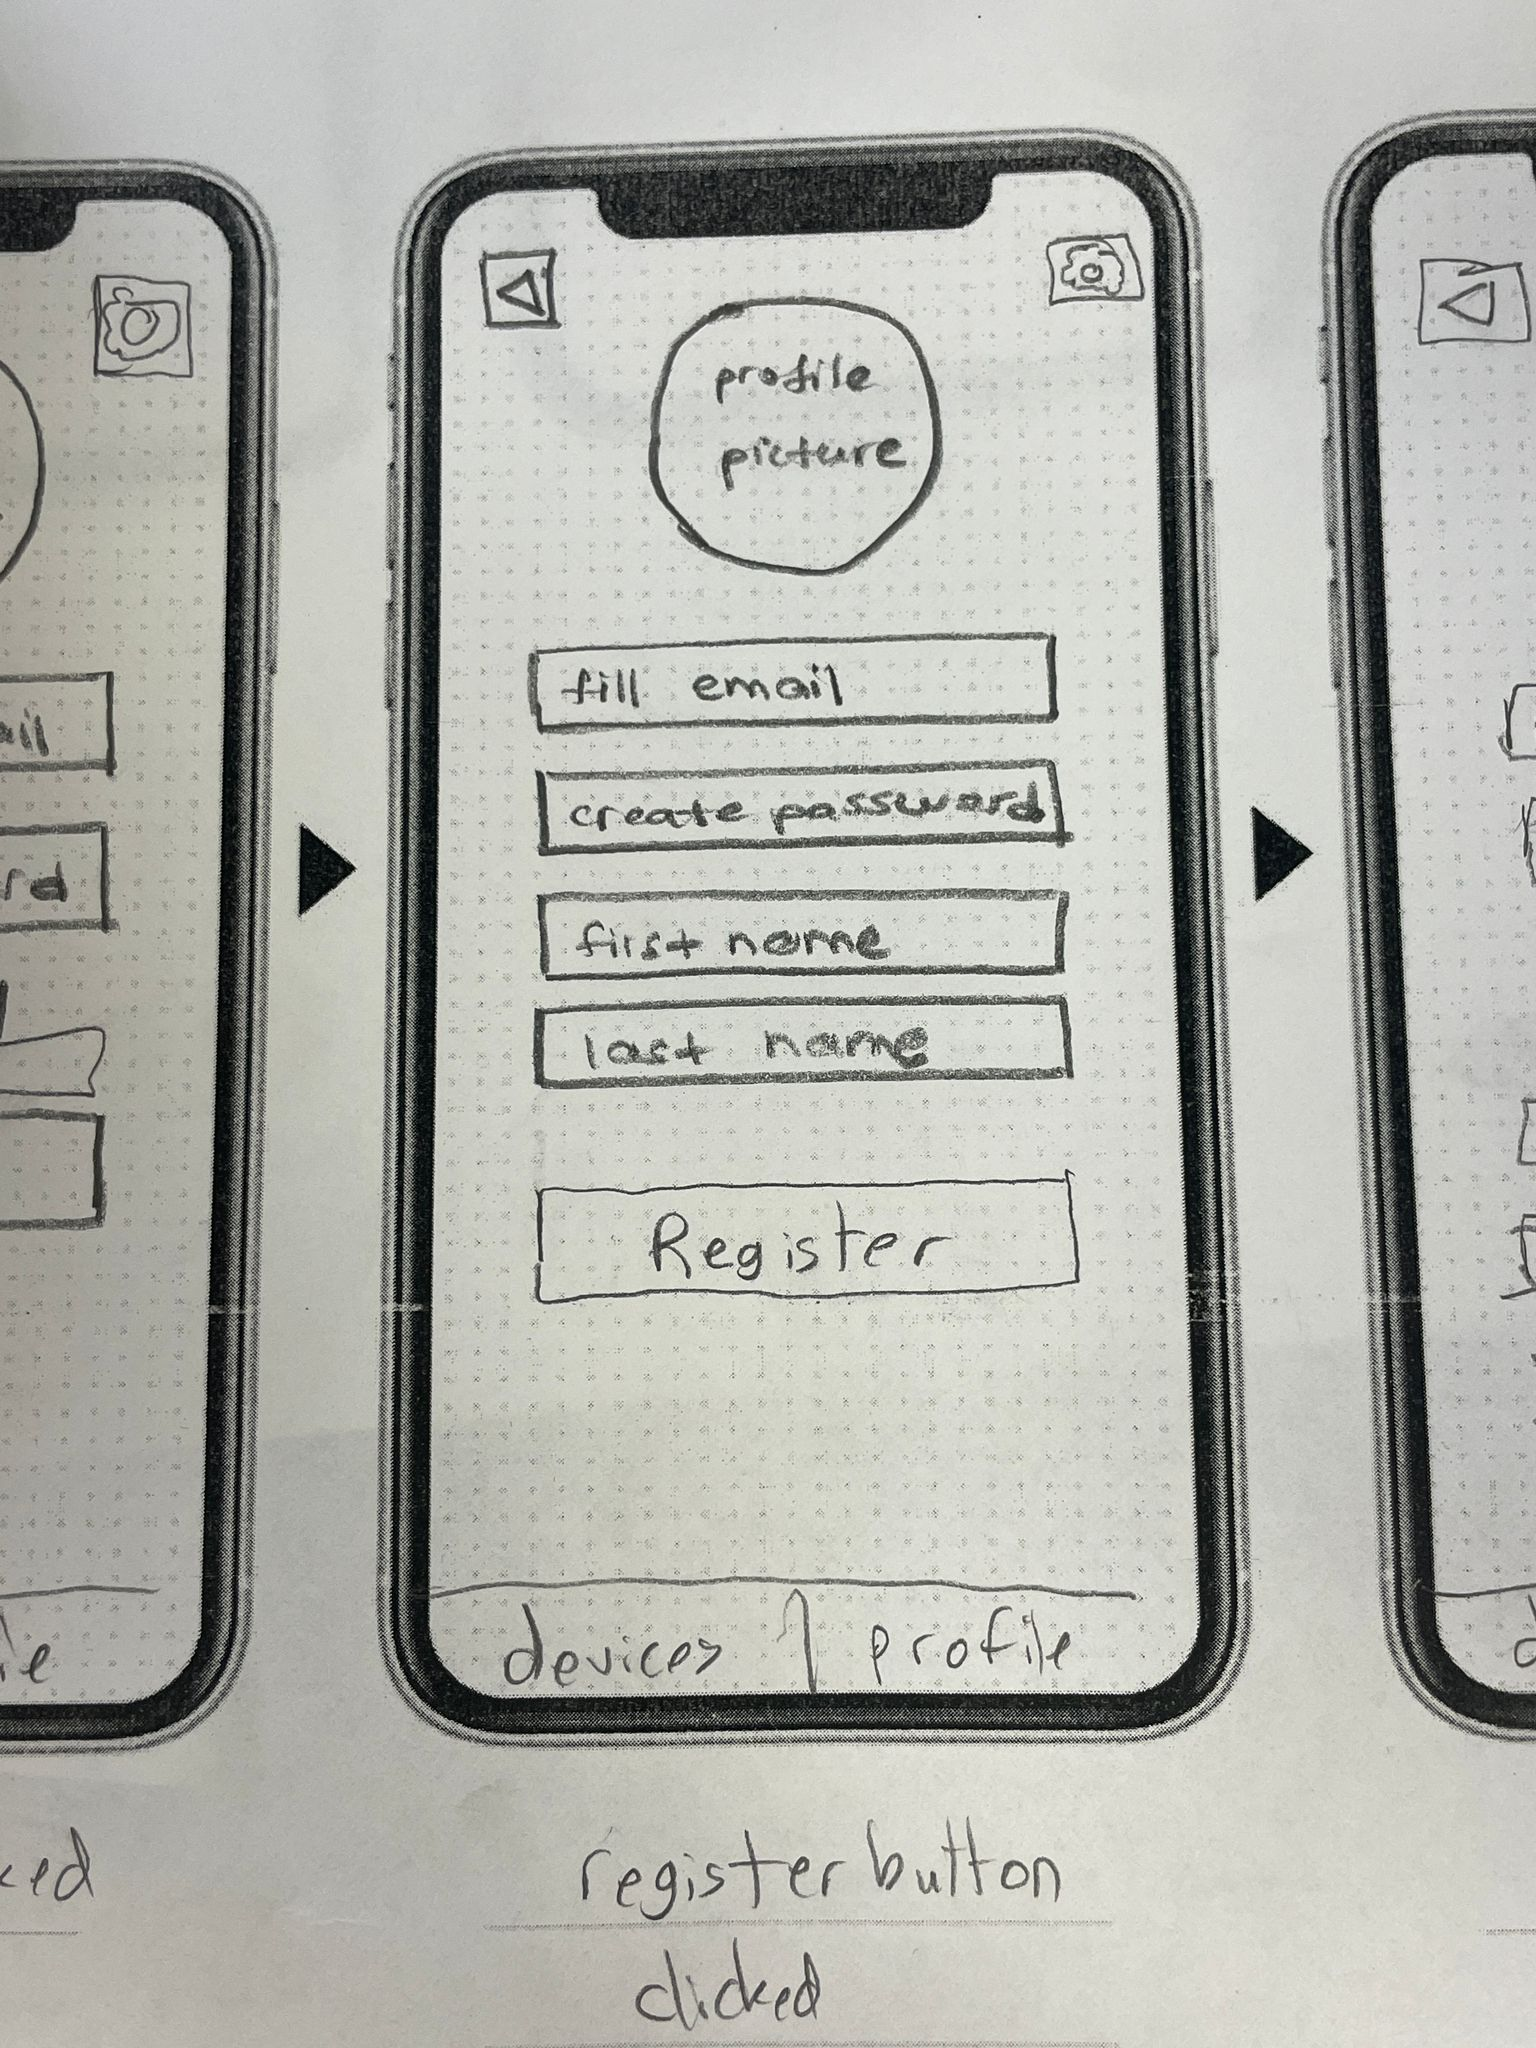
\includegraphics[width=0.42\textwidth]{profile/wireframe-register.jpeg}
  \caption{Register screen --- triggered by tapping ``Register'' on the login
    screen. Collects email, password, first name, and last name.}
  \label{fig:v1-register}
\end{figure}

\subsection{Forgot Password}

\begin{figure}[H]
  \centering
  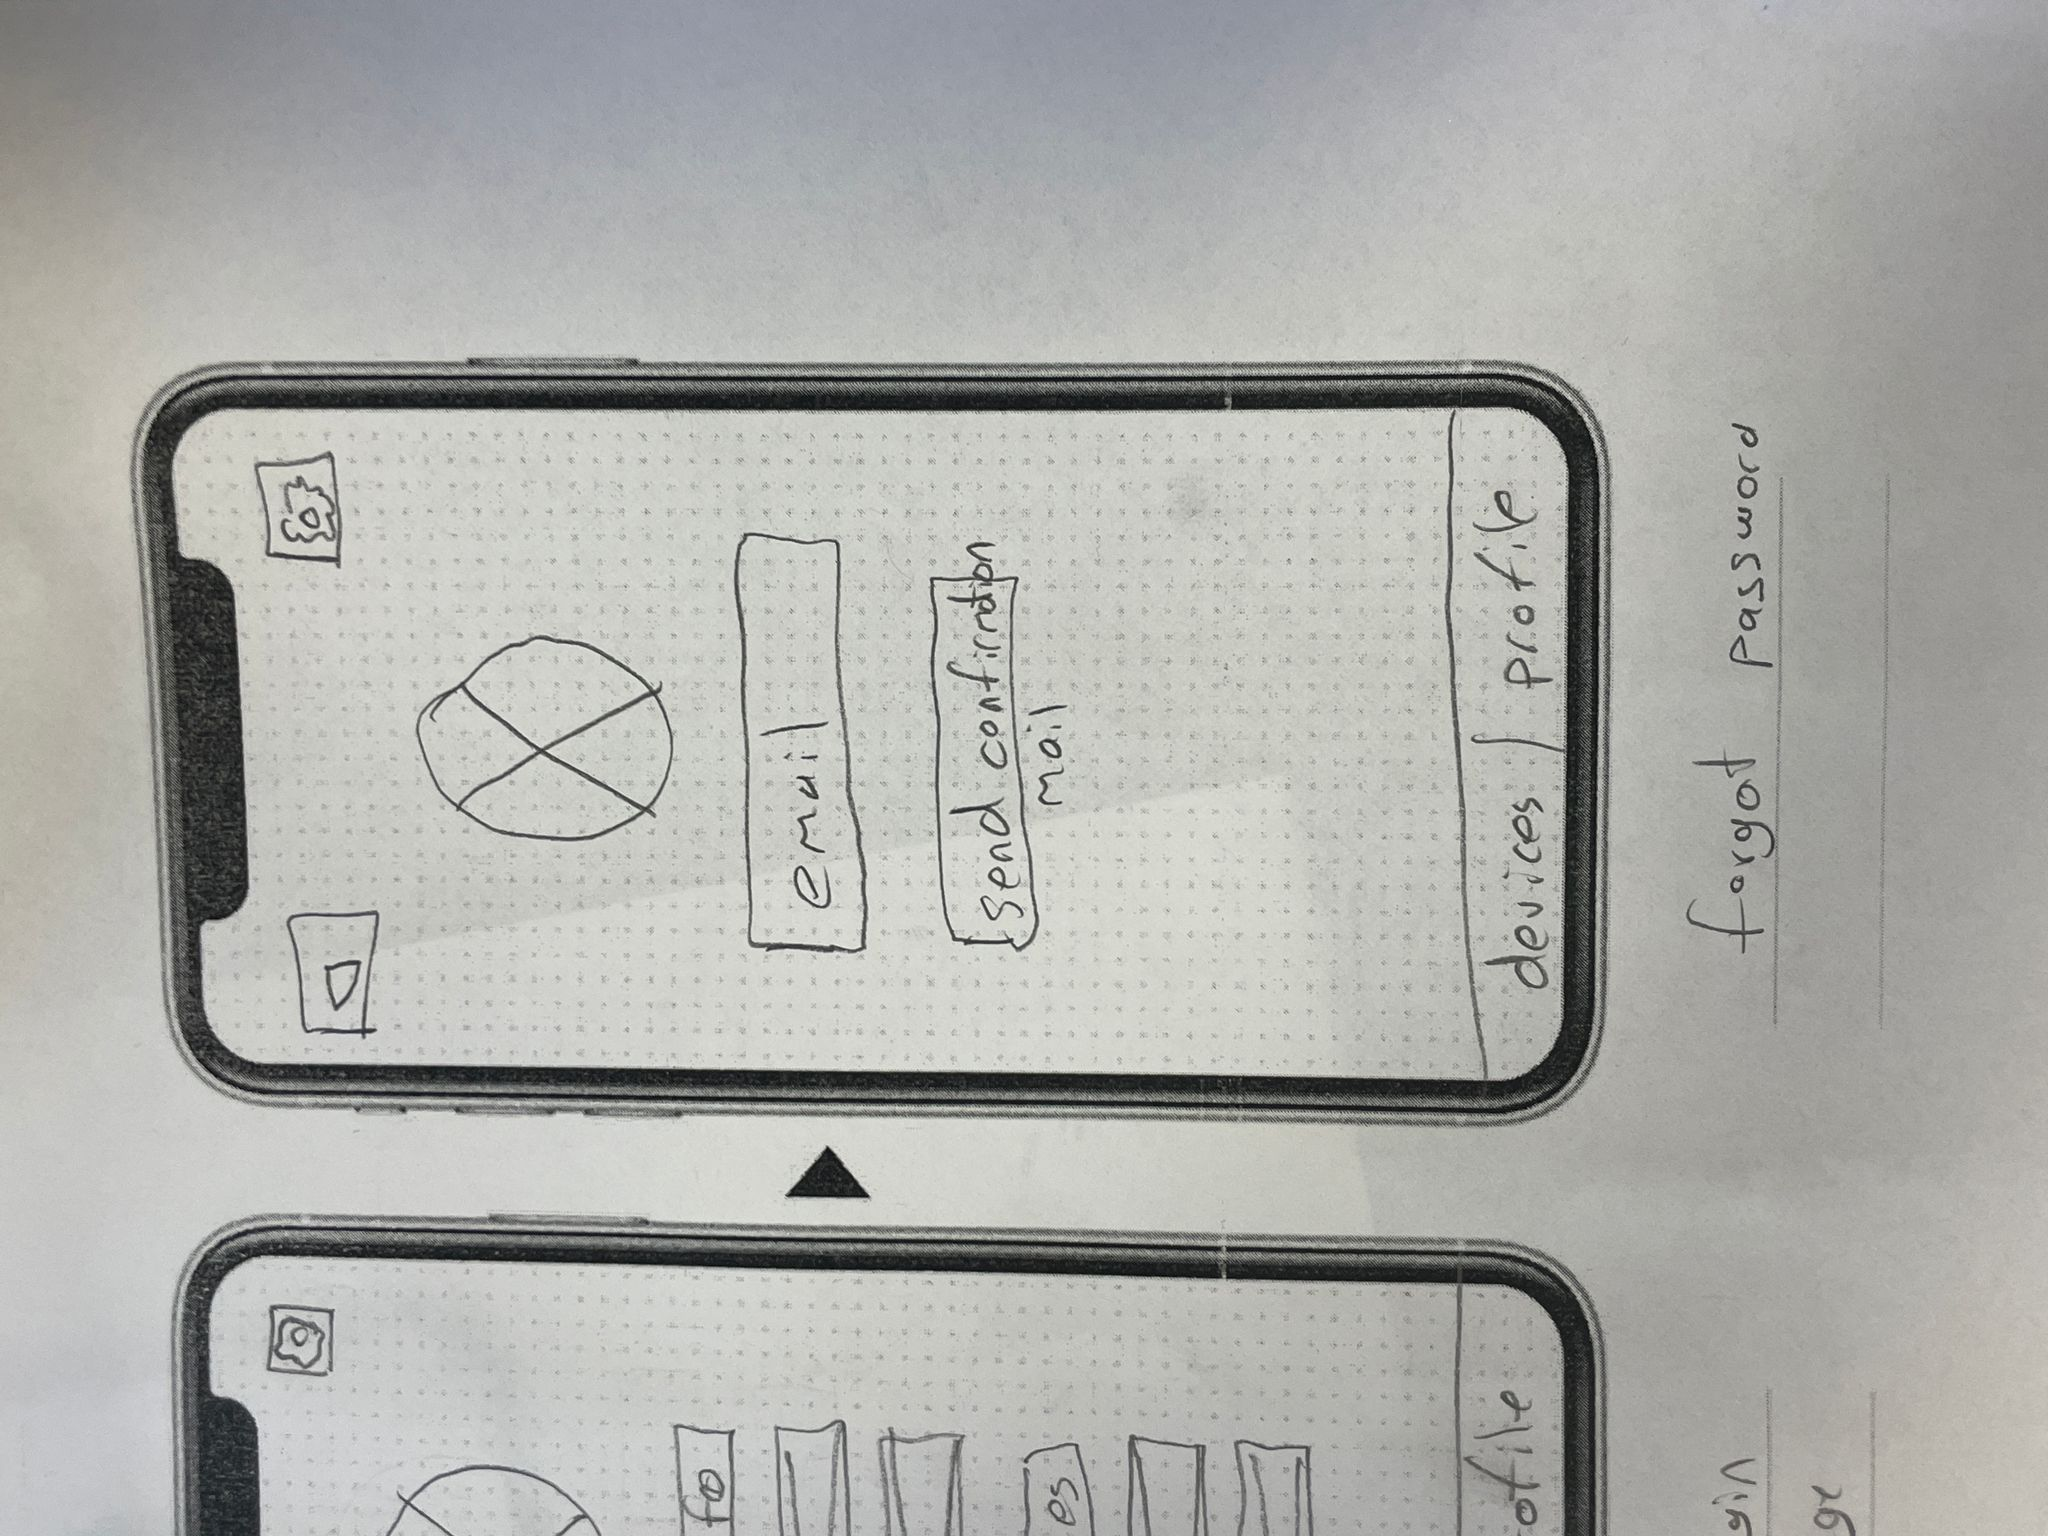
\includegraphics[angle=90, width=0.55\textwidth]{profile/wireframe-forgot-password-and-login.jpeg}
  \caption{Composite sheet: Forgot Password screen (top) with email input and
    ``Send Confirmation Mail'' CTA, alongside the Login screen (bottom) for
    context.}
  \label{fig:v1-forgot-pw}
\end{figure}

\subsection{Profile Overview \& Profile Menu}

\begin{figure}[H]
  \centering
  \begin{subfigure}[b]{0.45\textwidth}
    \centering
    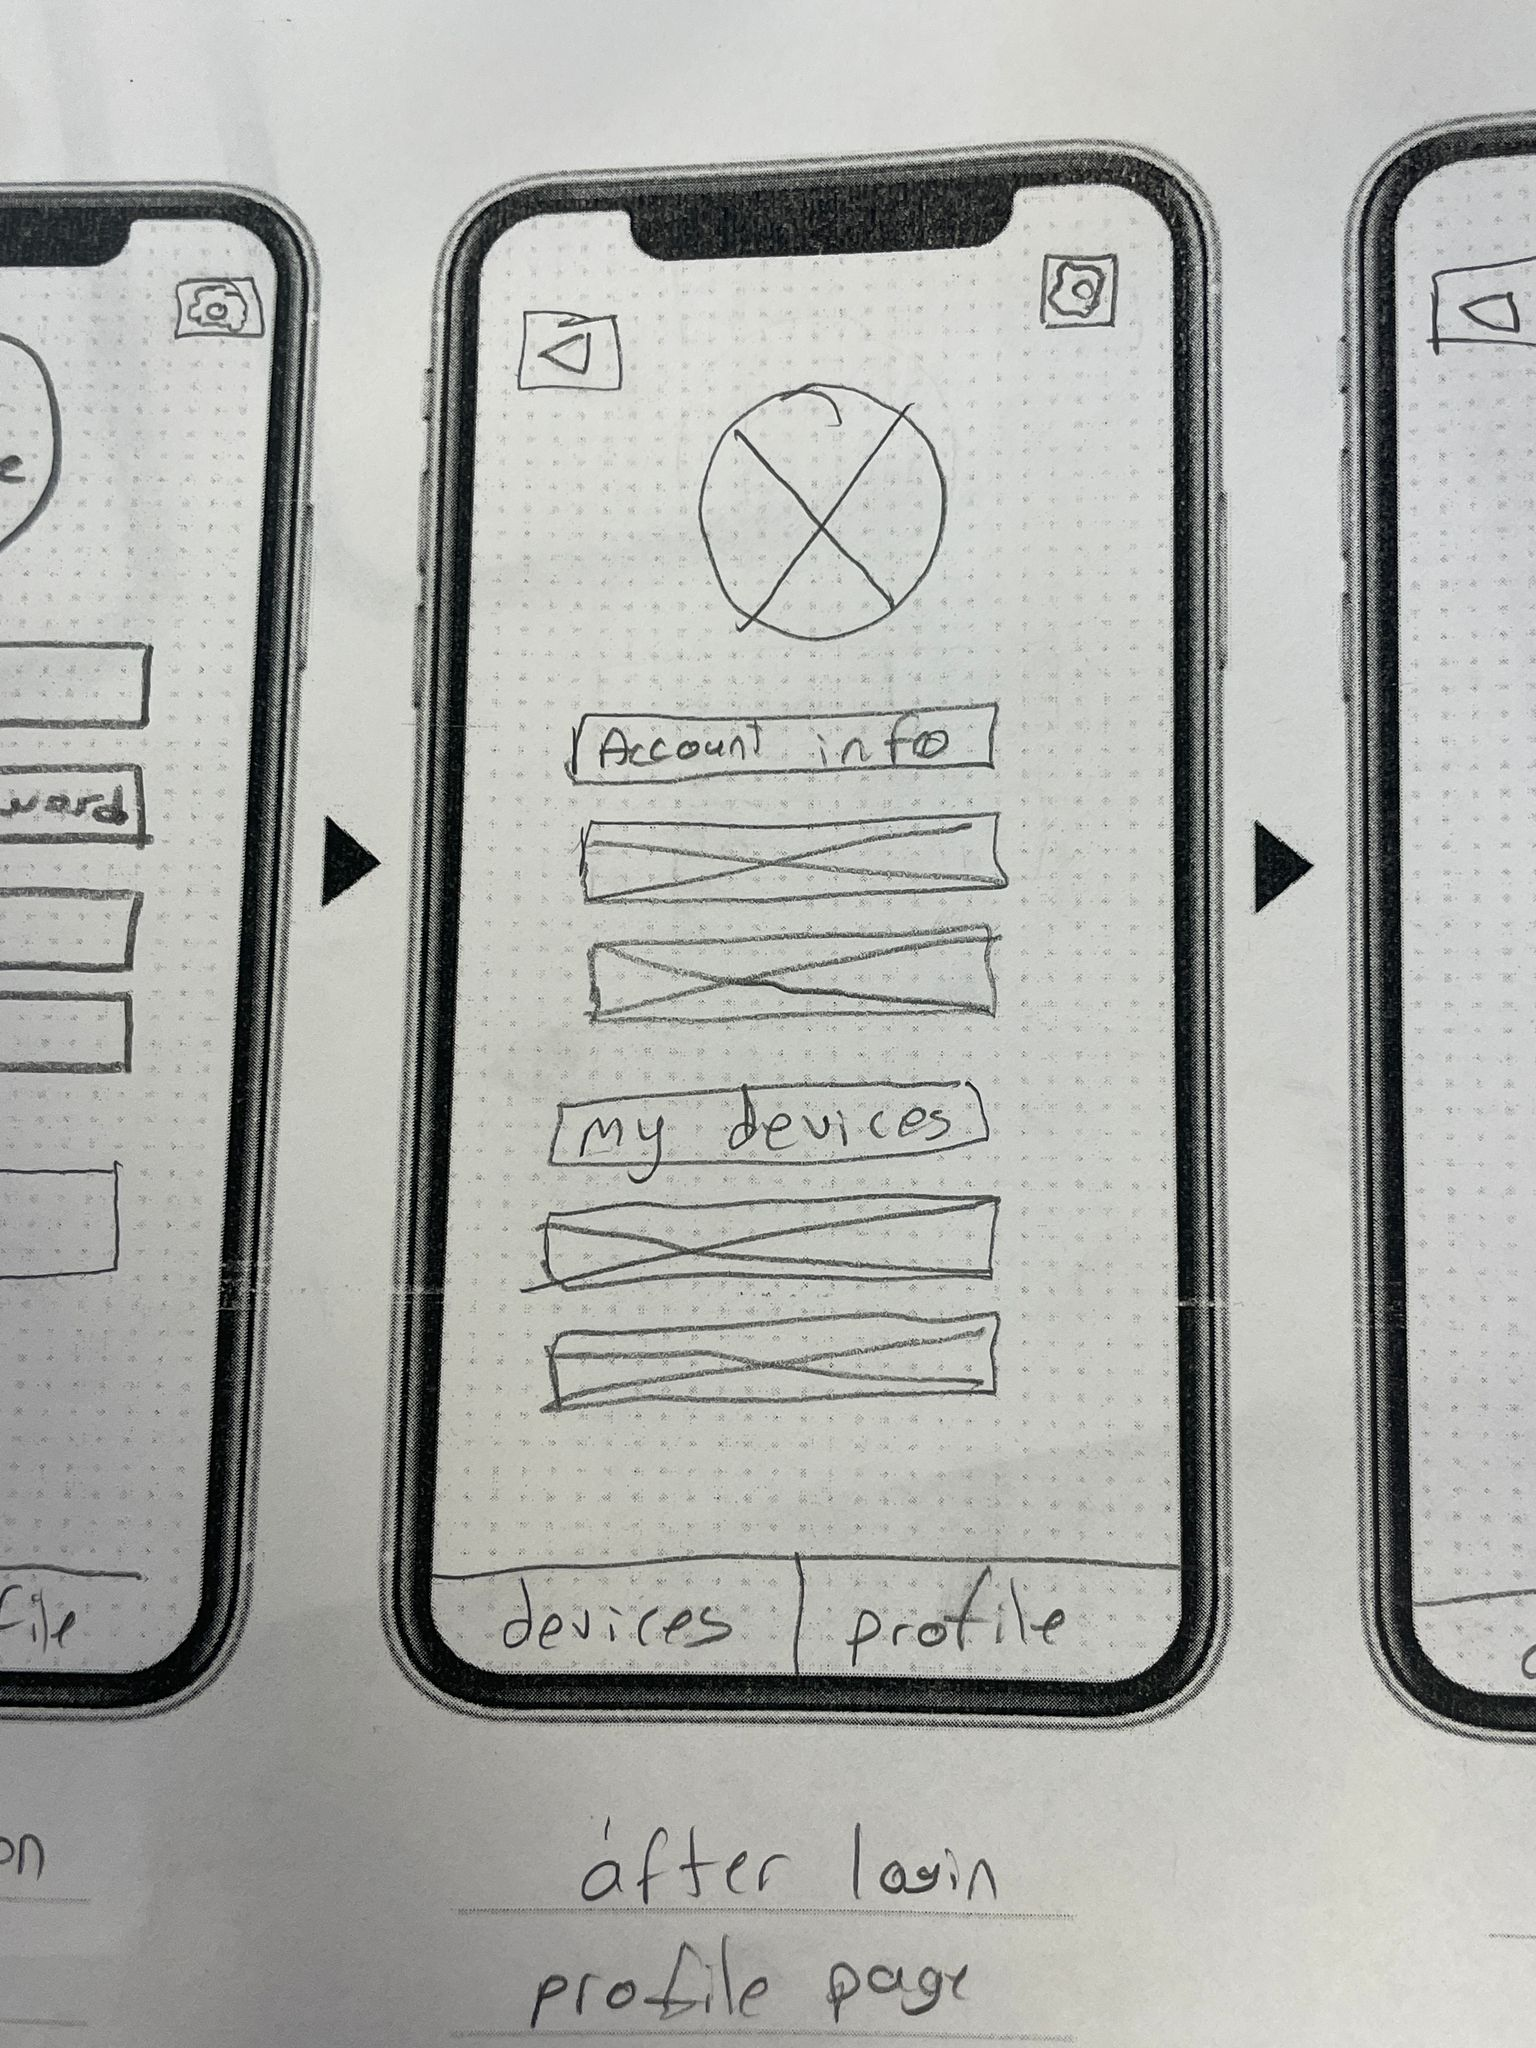
\includegraphics[width=\textwidth]{profile/wireframe-profile-overview.jpeg}
    \caption{Profile overview layout.}
    \label{fig:v1-profile-overview}
  \end{subfigure}
  \hfill
  \begin{subfigure}[b]{0.45\textwidth}
    \centering
    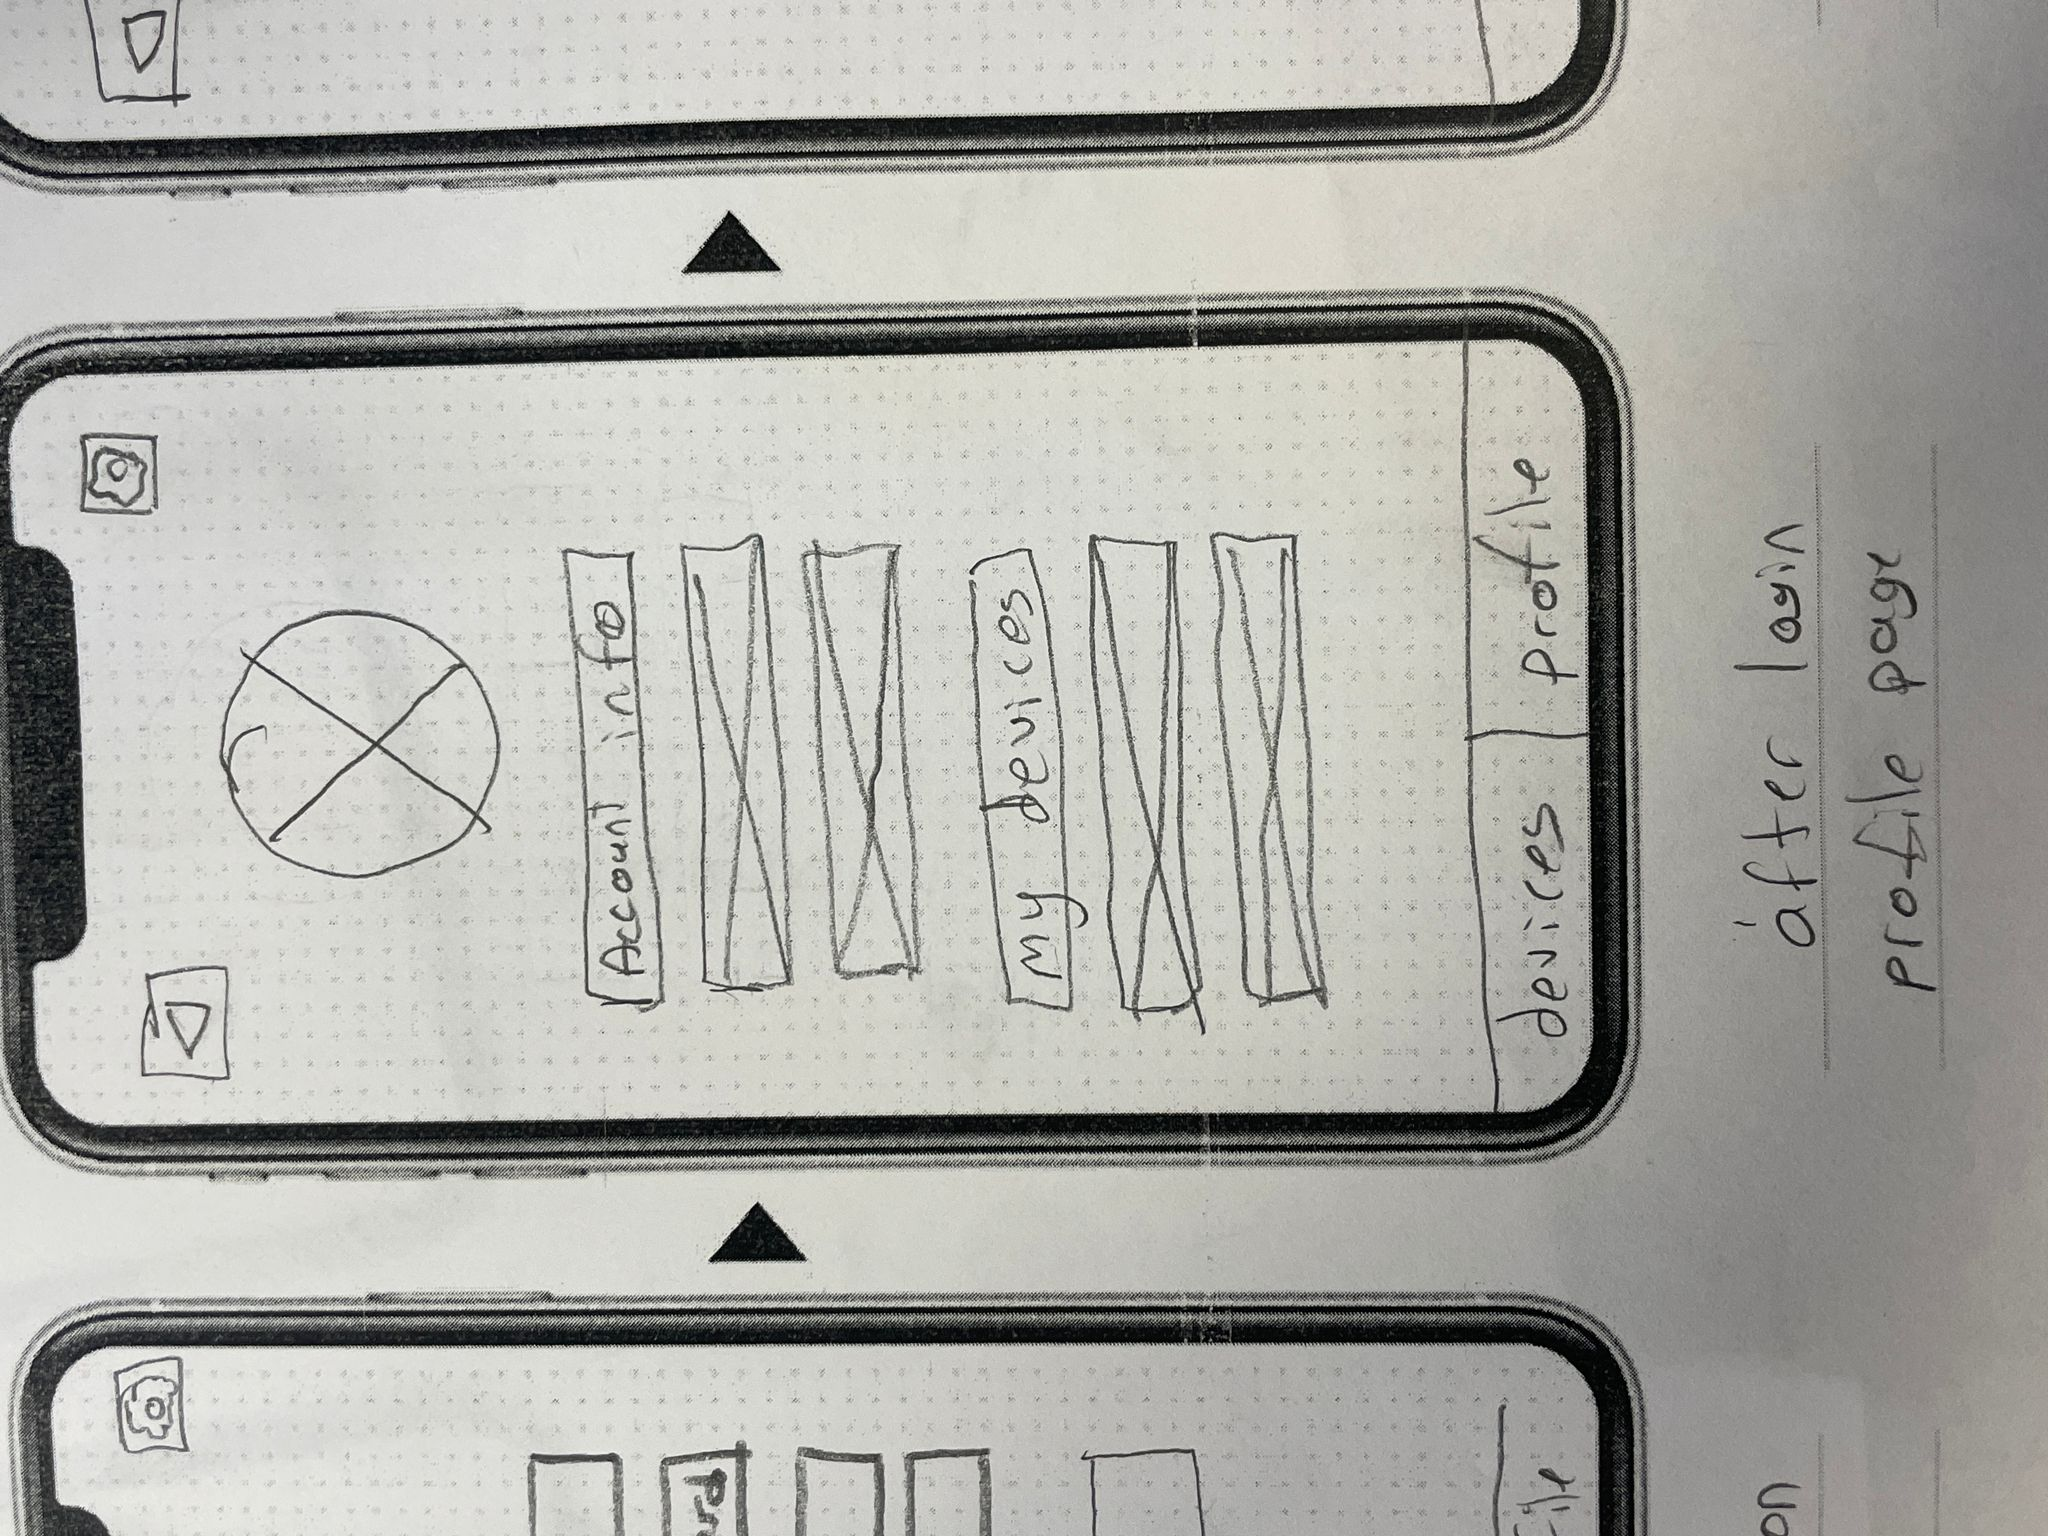
\includegraphics[angle=90, width=\textwidth]{profile/wireframe-profile-menu.jpeg}
    \caption{Profile menu list layout.}
    \label{fig:v1-profile-menu}
  \end{subfigure}
  \caption{Two after-login profile layouts explored in Version~1.
    The overview (left) uses sections; the menu (right) uses a simple vertical
    list. The menu list was preferred for its scannability and scalability.}
  \label{fig:v1-profile-both}
\end{figure}

% -------------------------------------------------------
\section{Settings Screens}
% -------------------------------------------------------

\subsection{General Settings}

\begin{figure}[H]
  \centering
  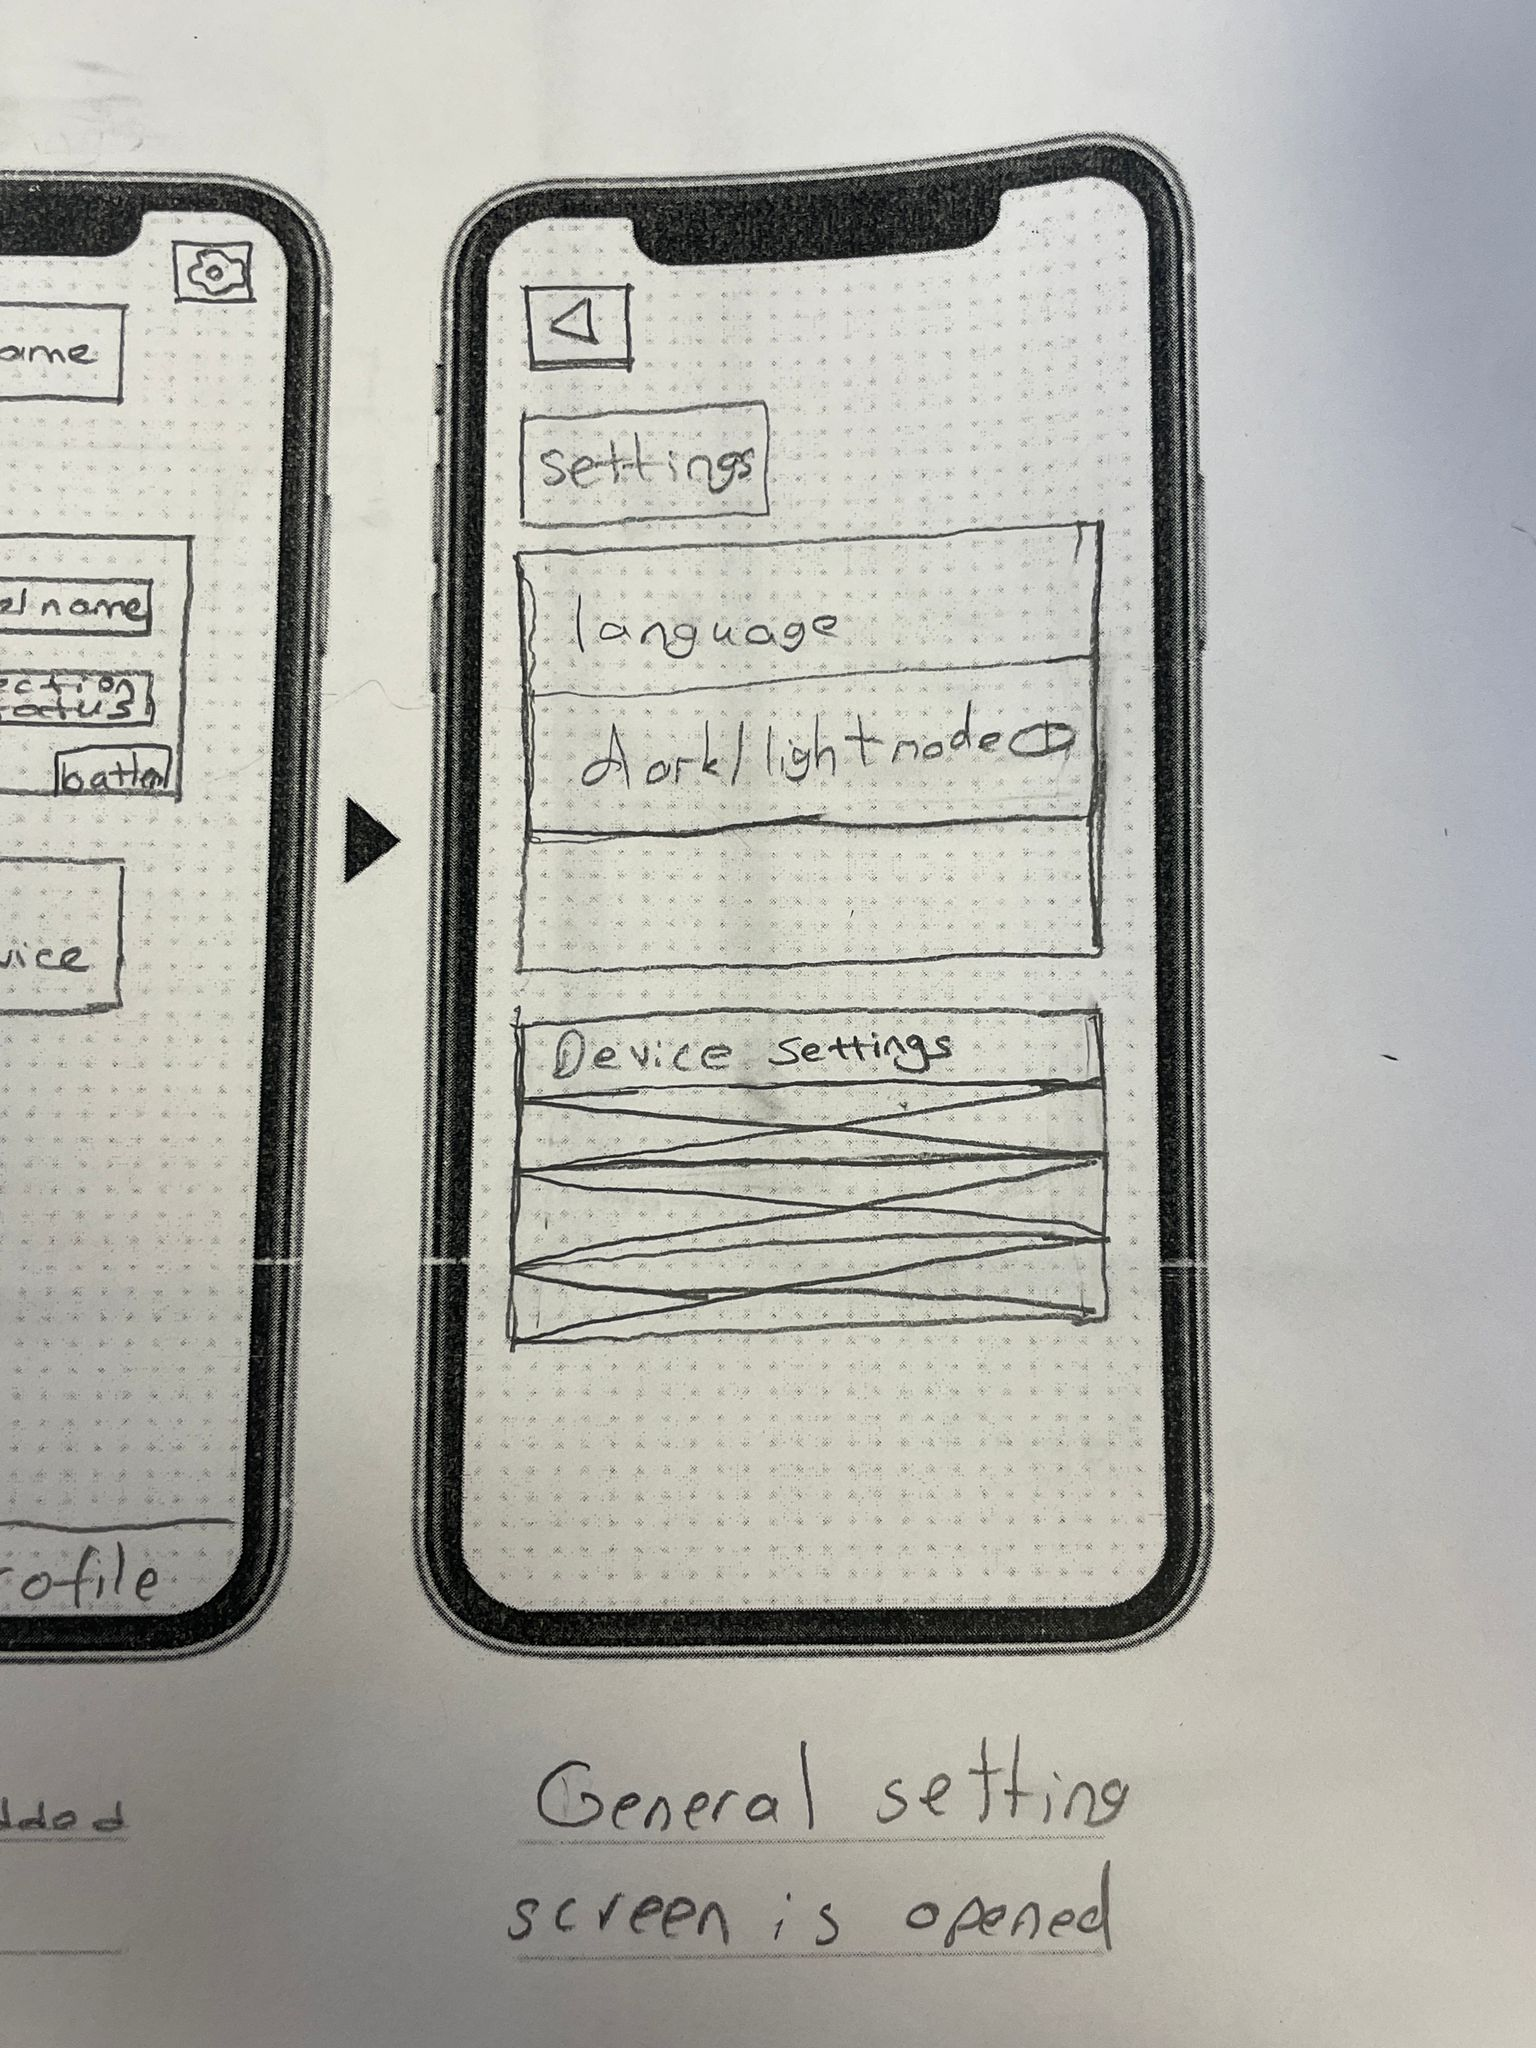
\includegraphics[width=0.42\textwidth]{settings/wireframe-settings-general.jpeg}
  \caption{General settings: Language row, Dark/Light Mode toggle, and a Device
    Settings section that groups per-device configuration.}
  \label{fig:v1-settings-general}
\end{figure}

\subsection{Device Detail Settings}

\begin{figure}[H]
  \centering
  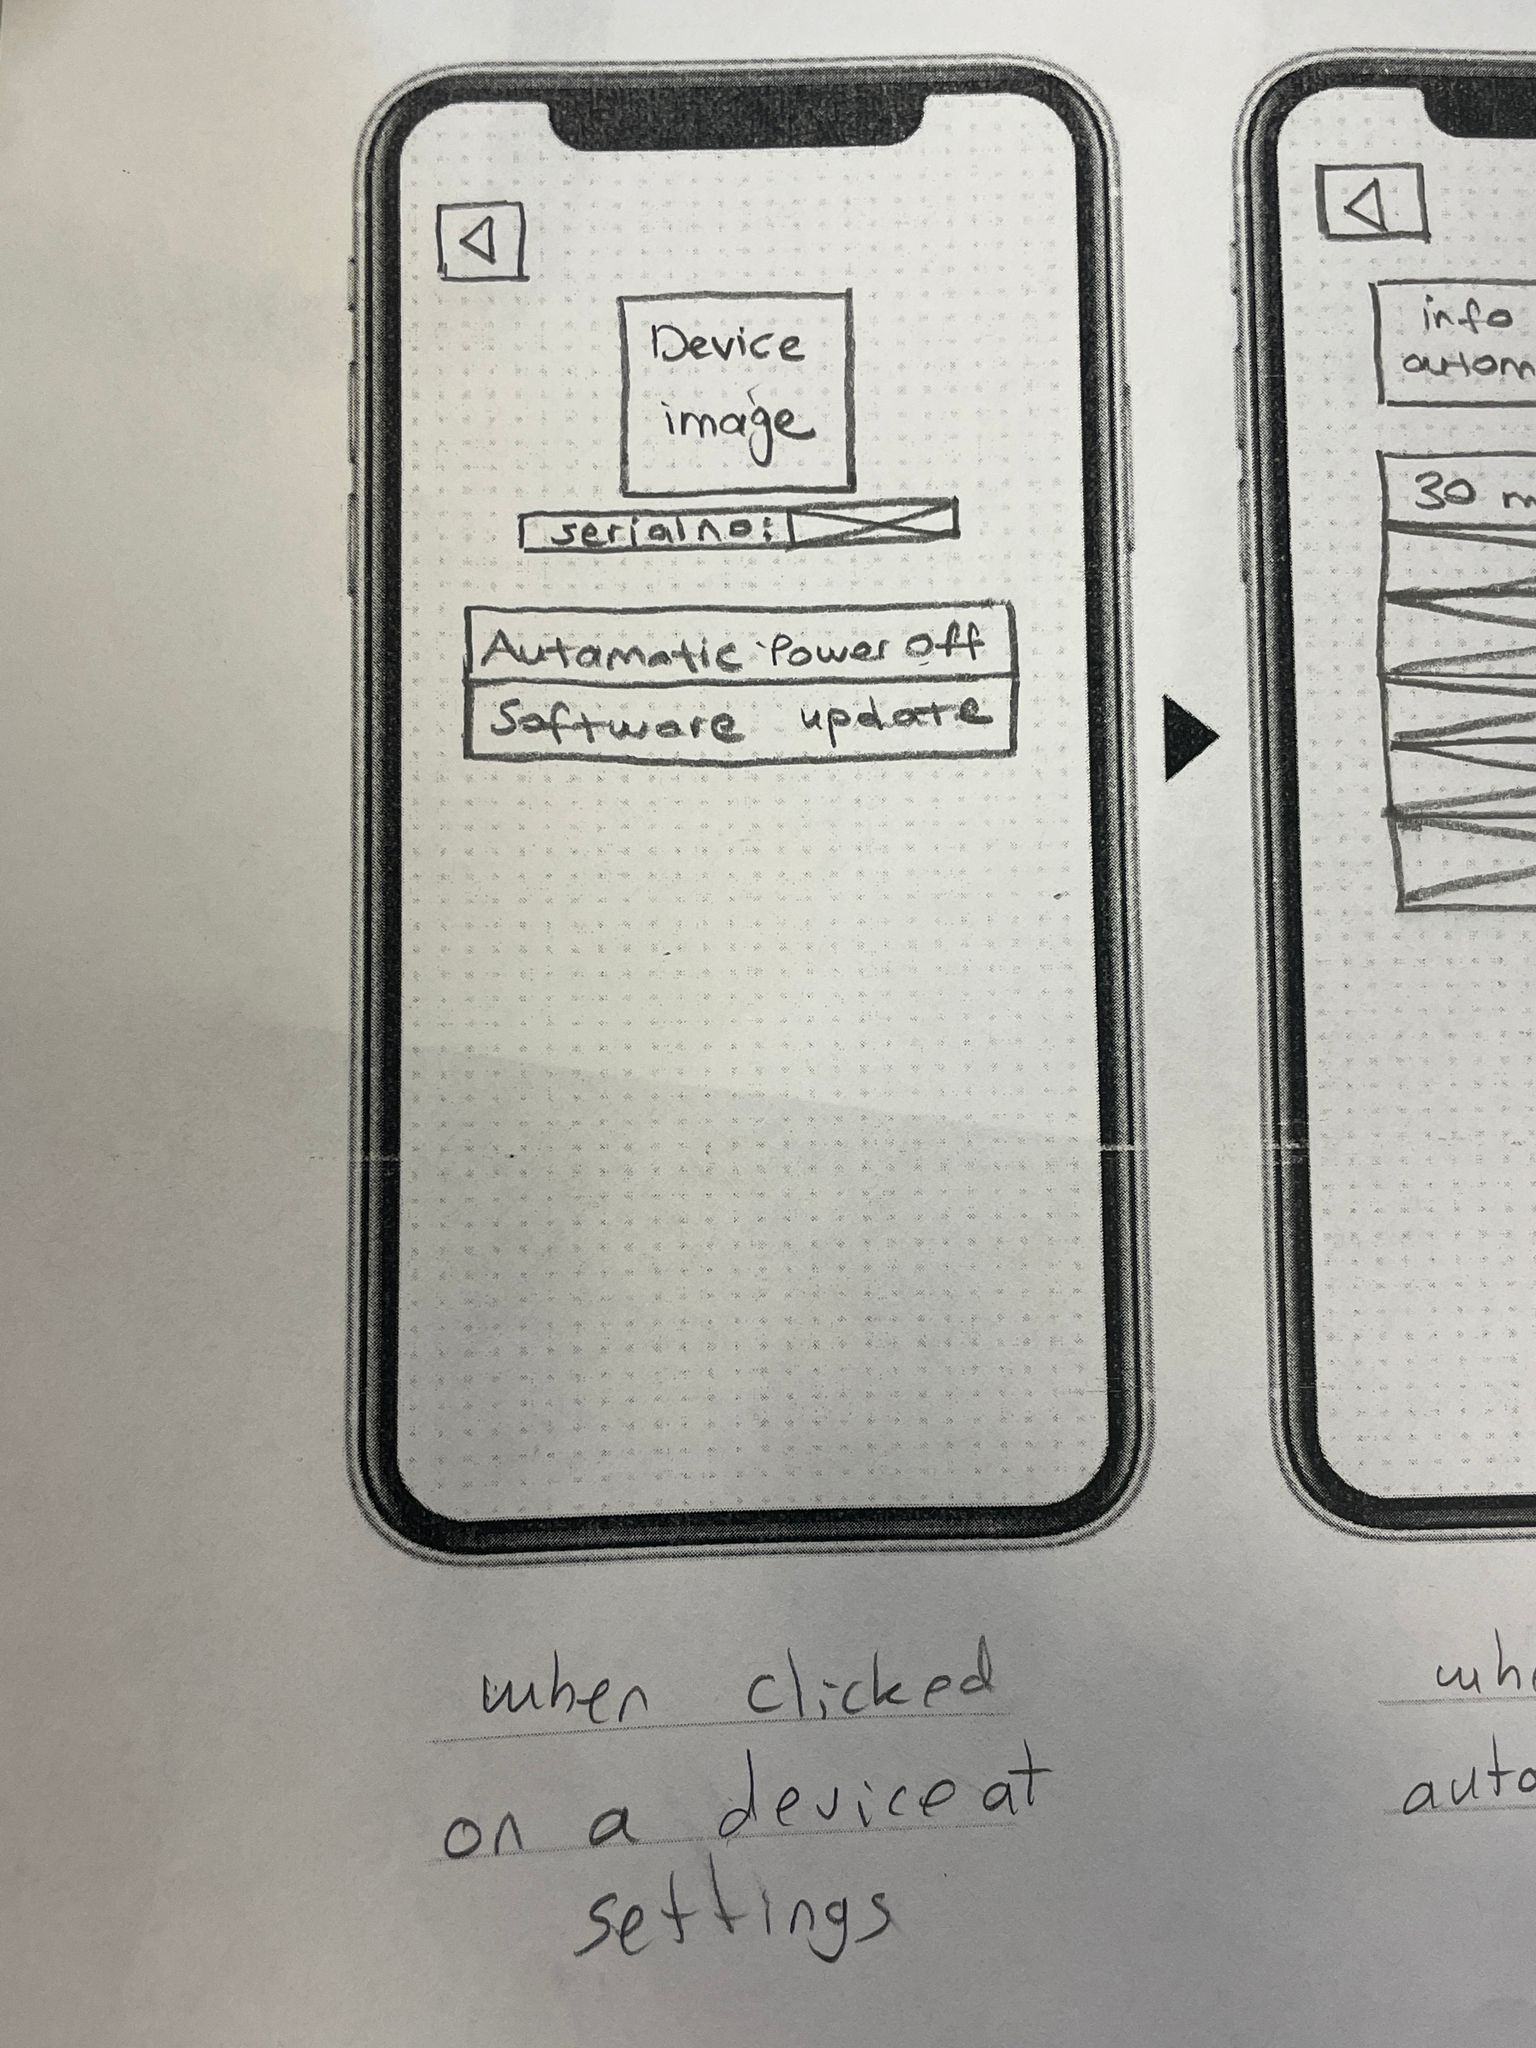
\includegraphics[width=0.42\textwidth]{settings/wireframe-settings-device-detail.jpeg}
  \caption{Device detail settings: device image, serial number, and action rows
    for Automatic Power Off and Software Update.}
  \label{fig:v1-settings-device-detail}
\end{figure}

\subsection{Automatic Power-Off}

\begin{figure}[H]
  \centering
  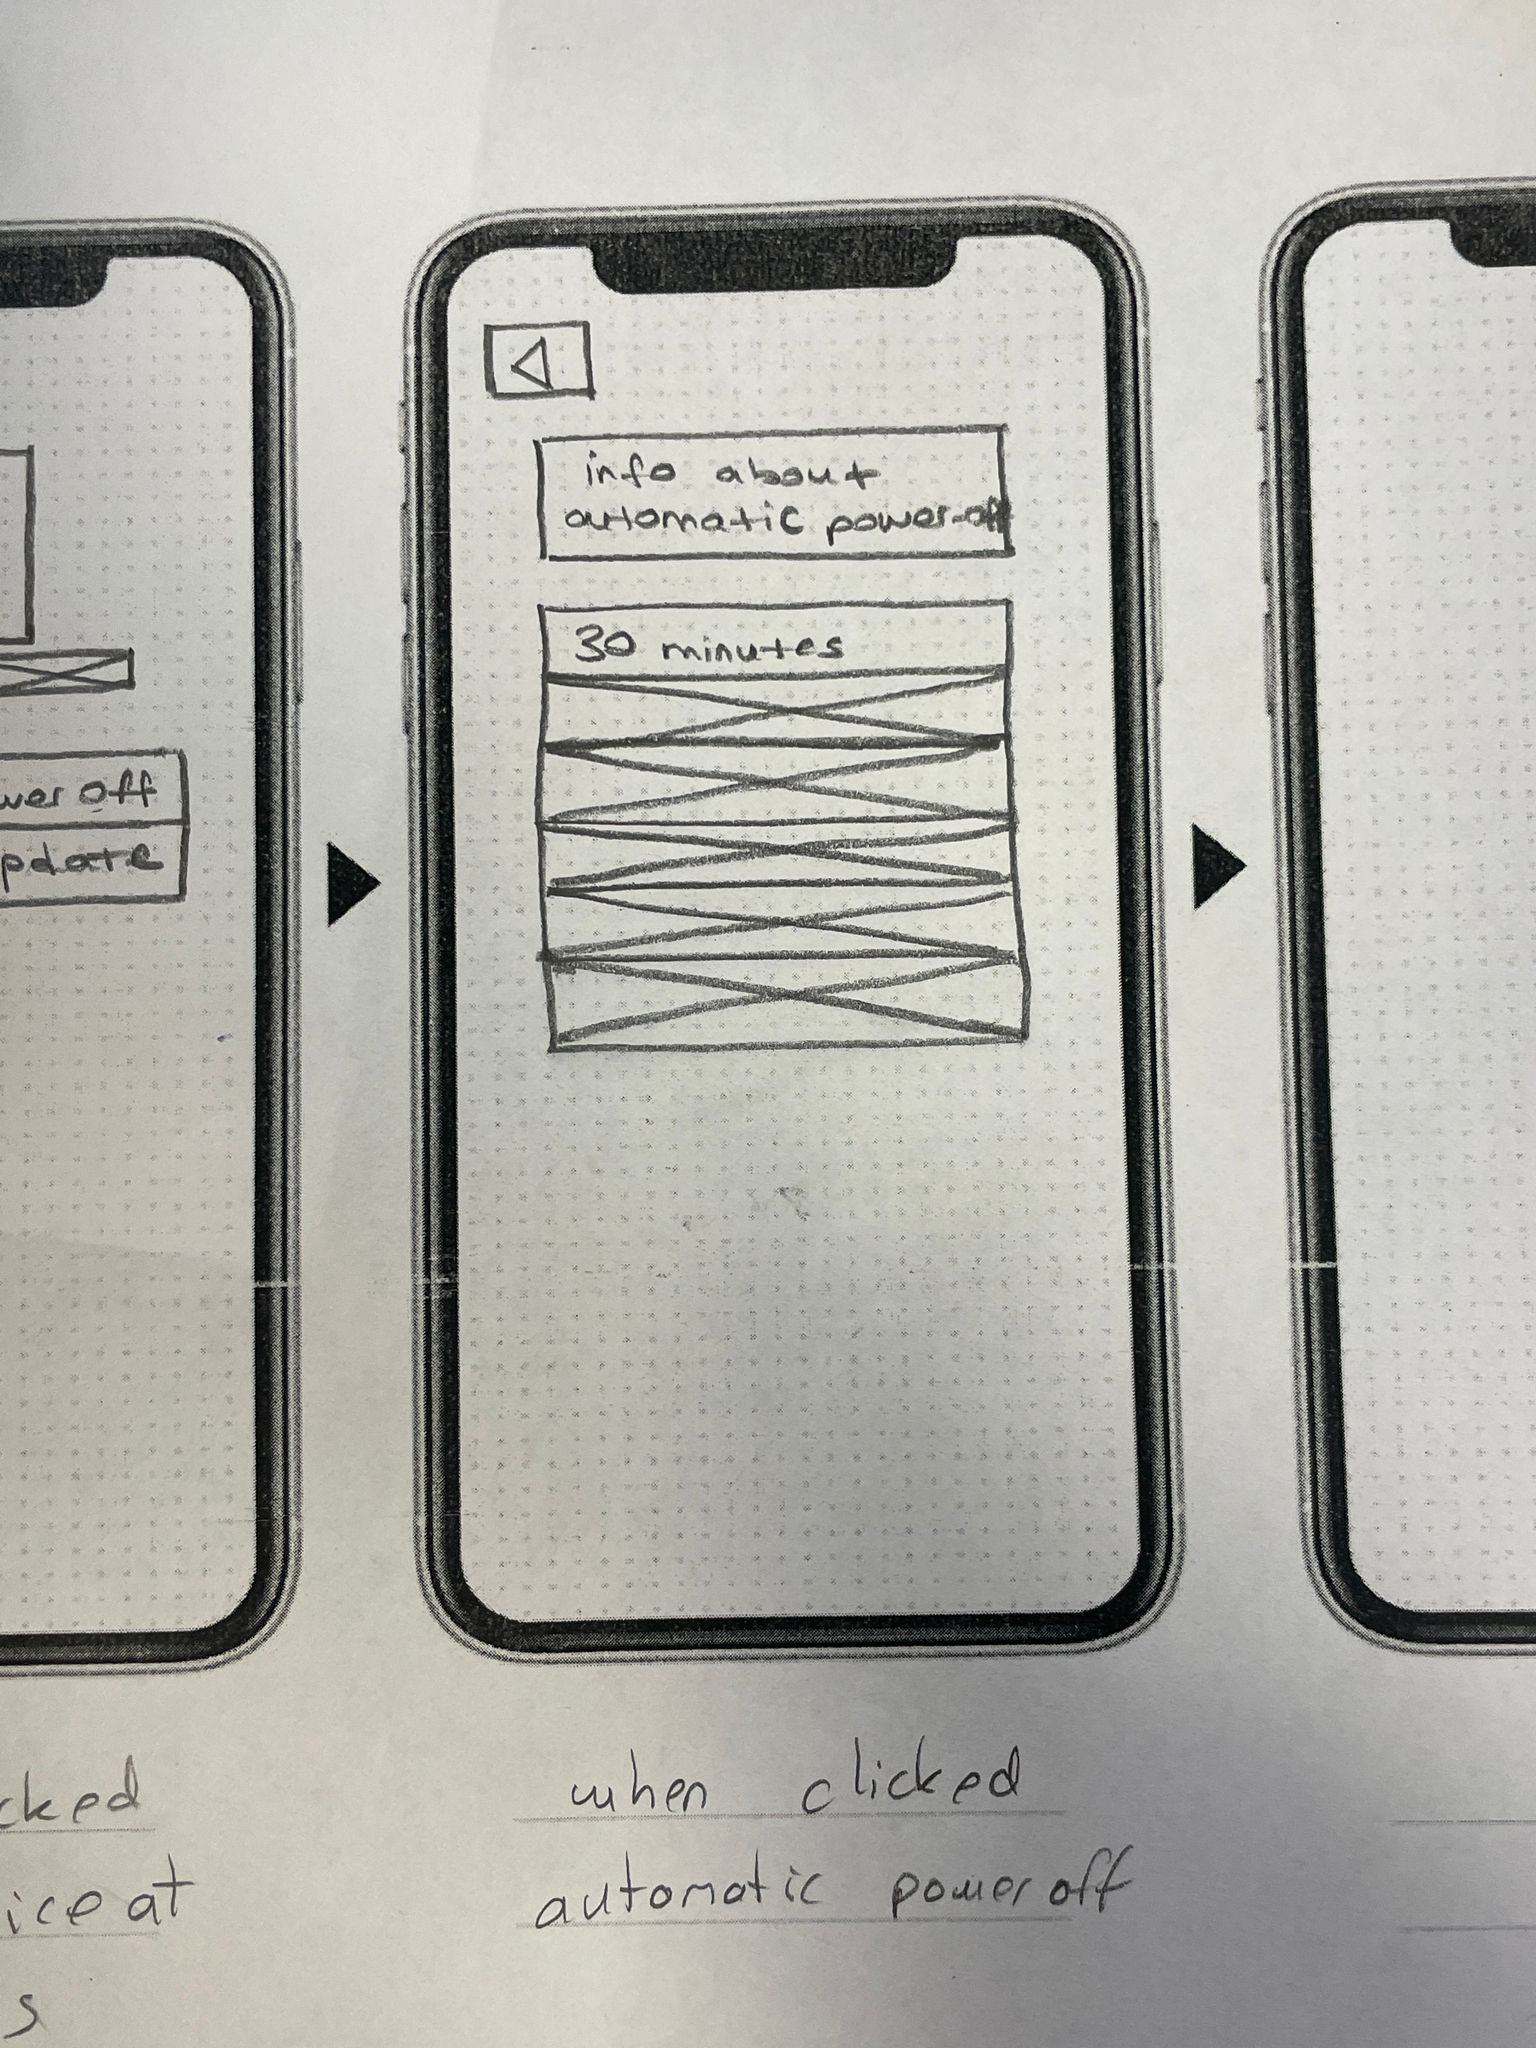
\includegraphics[width=0.42\textwidth]{settings/wireframe-settings-automatic-power-off.jpeg}
  \caption{Automatic Power-Off picker: a dedicated screen with an information
    block and a list of duration options (e.g.\ 30 minutes).}
  \label{fig:v1-power-off}
\end{figure}

% -------------------------------------------------------
\section{Version 1 Flowsheets}
% -------------------------------------------------------

Flowsheets place multiple screens on one page to verify that transitions between
states are coherent before moving to the next design version.

\subsection{Add Device \& Settings Flow}

\begin{figure}[H]
  \centering
  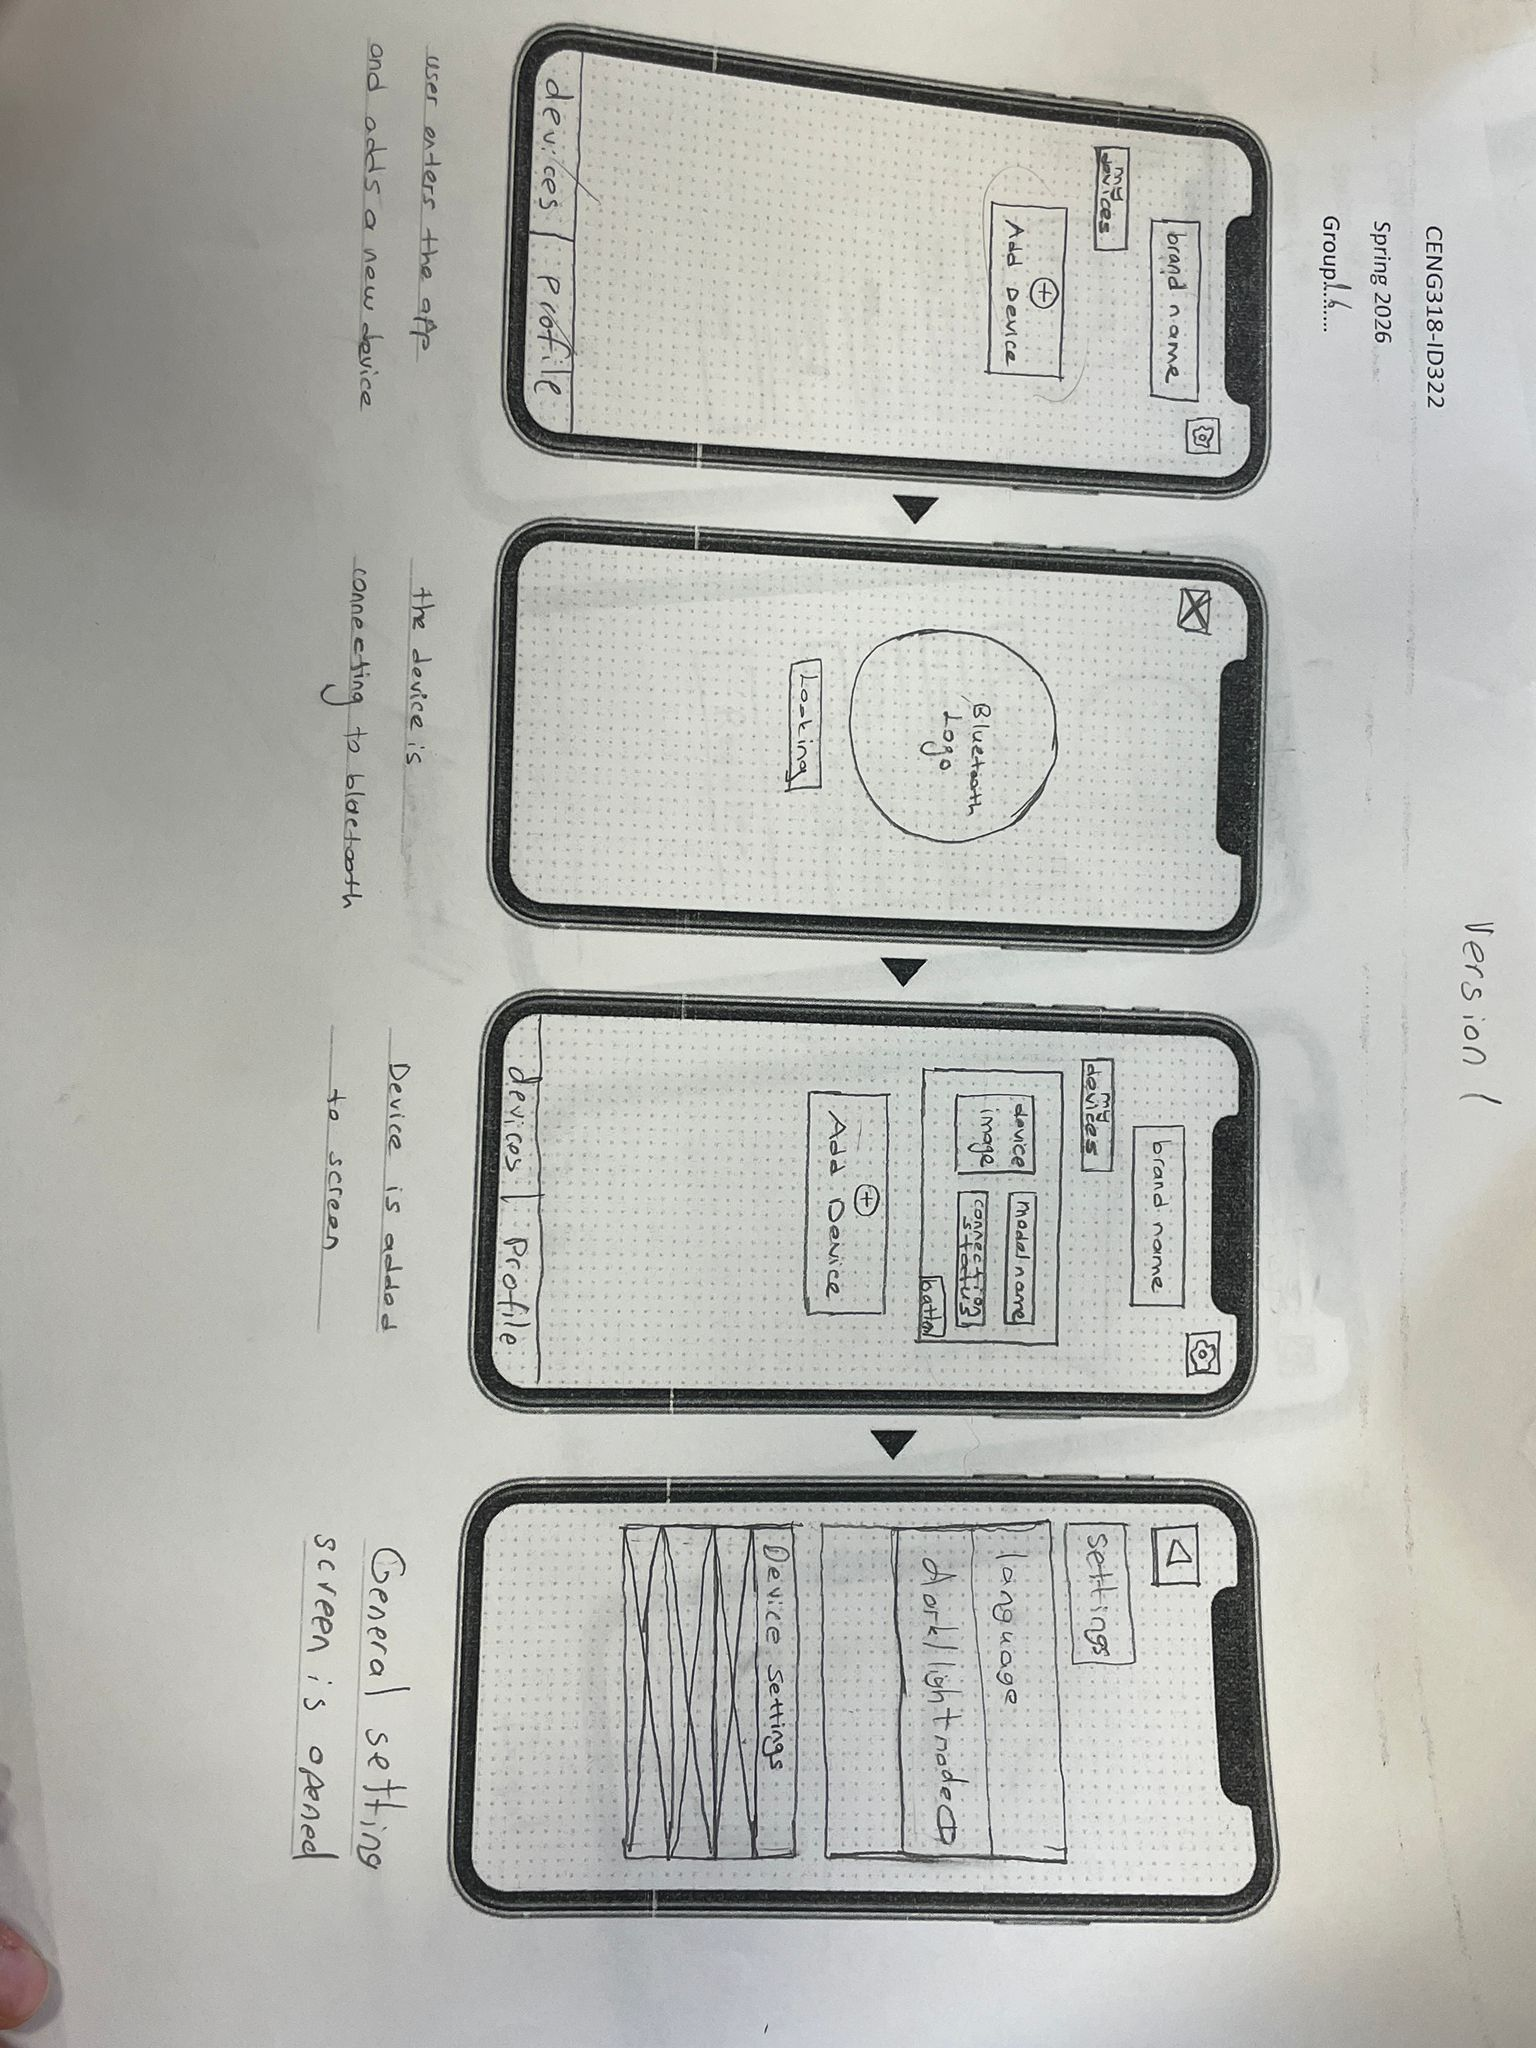
\includegraphics[width=0.82\textwidth]{flowsheets/flowsheet-add-device-and-settings.jpeg}
  \caption{Four-frame flowsheet: (1) empty home $\to$ (2) Bluetooth searching
    $\to$ (3) populated home $\to$ (4) General Settings. Handwritten notes
    annotate each transition.}
  \label{fig:v1-flow-add-device}
\end{figure}

\subsection{Authentication \& Profile Flow}

\begin{figure}[H]
  \centering
  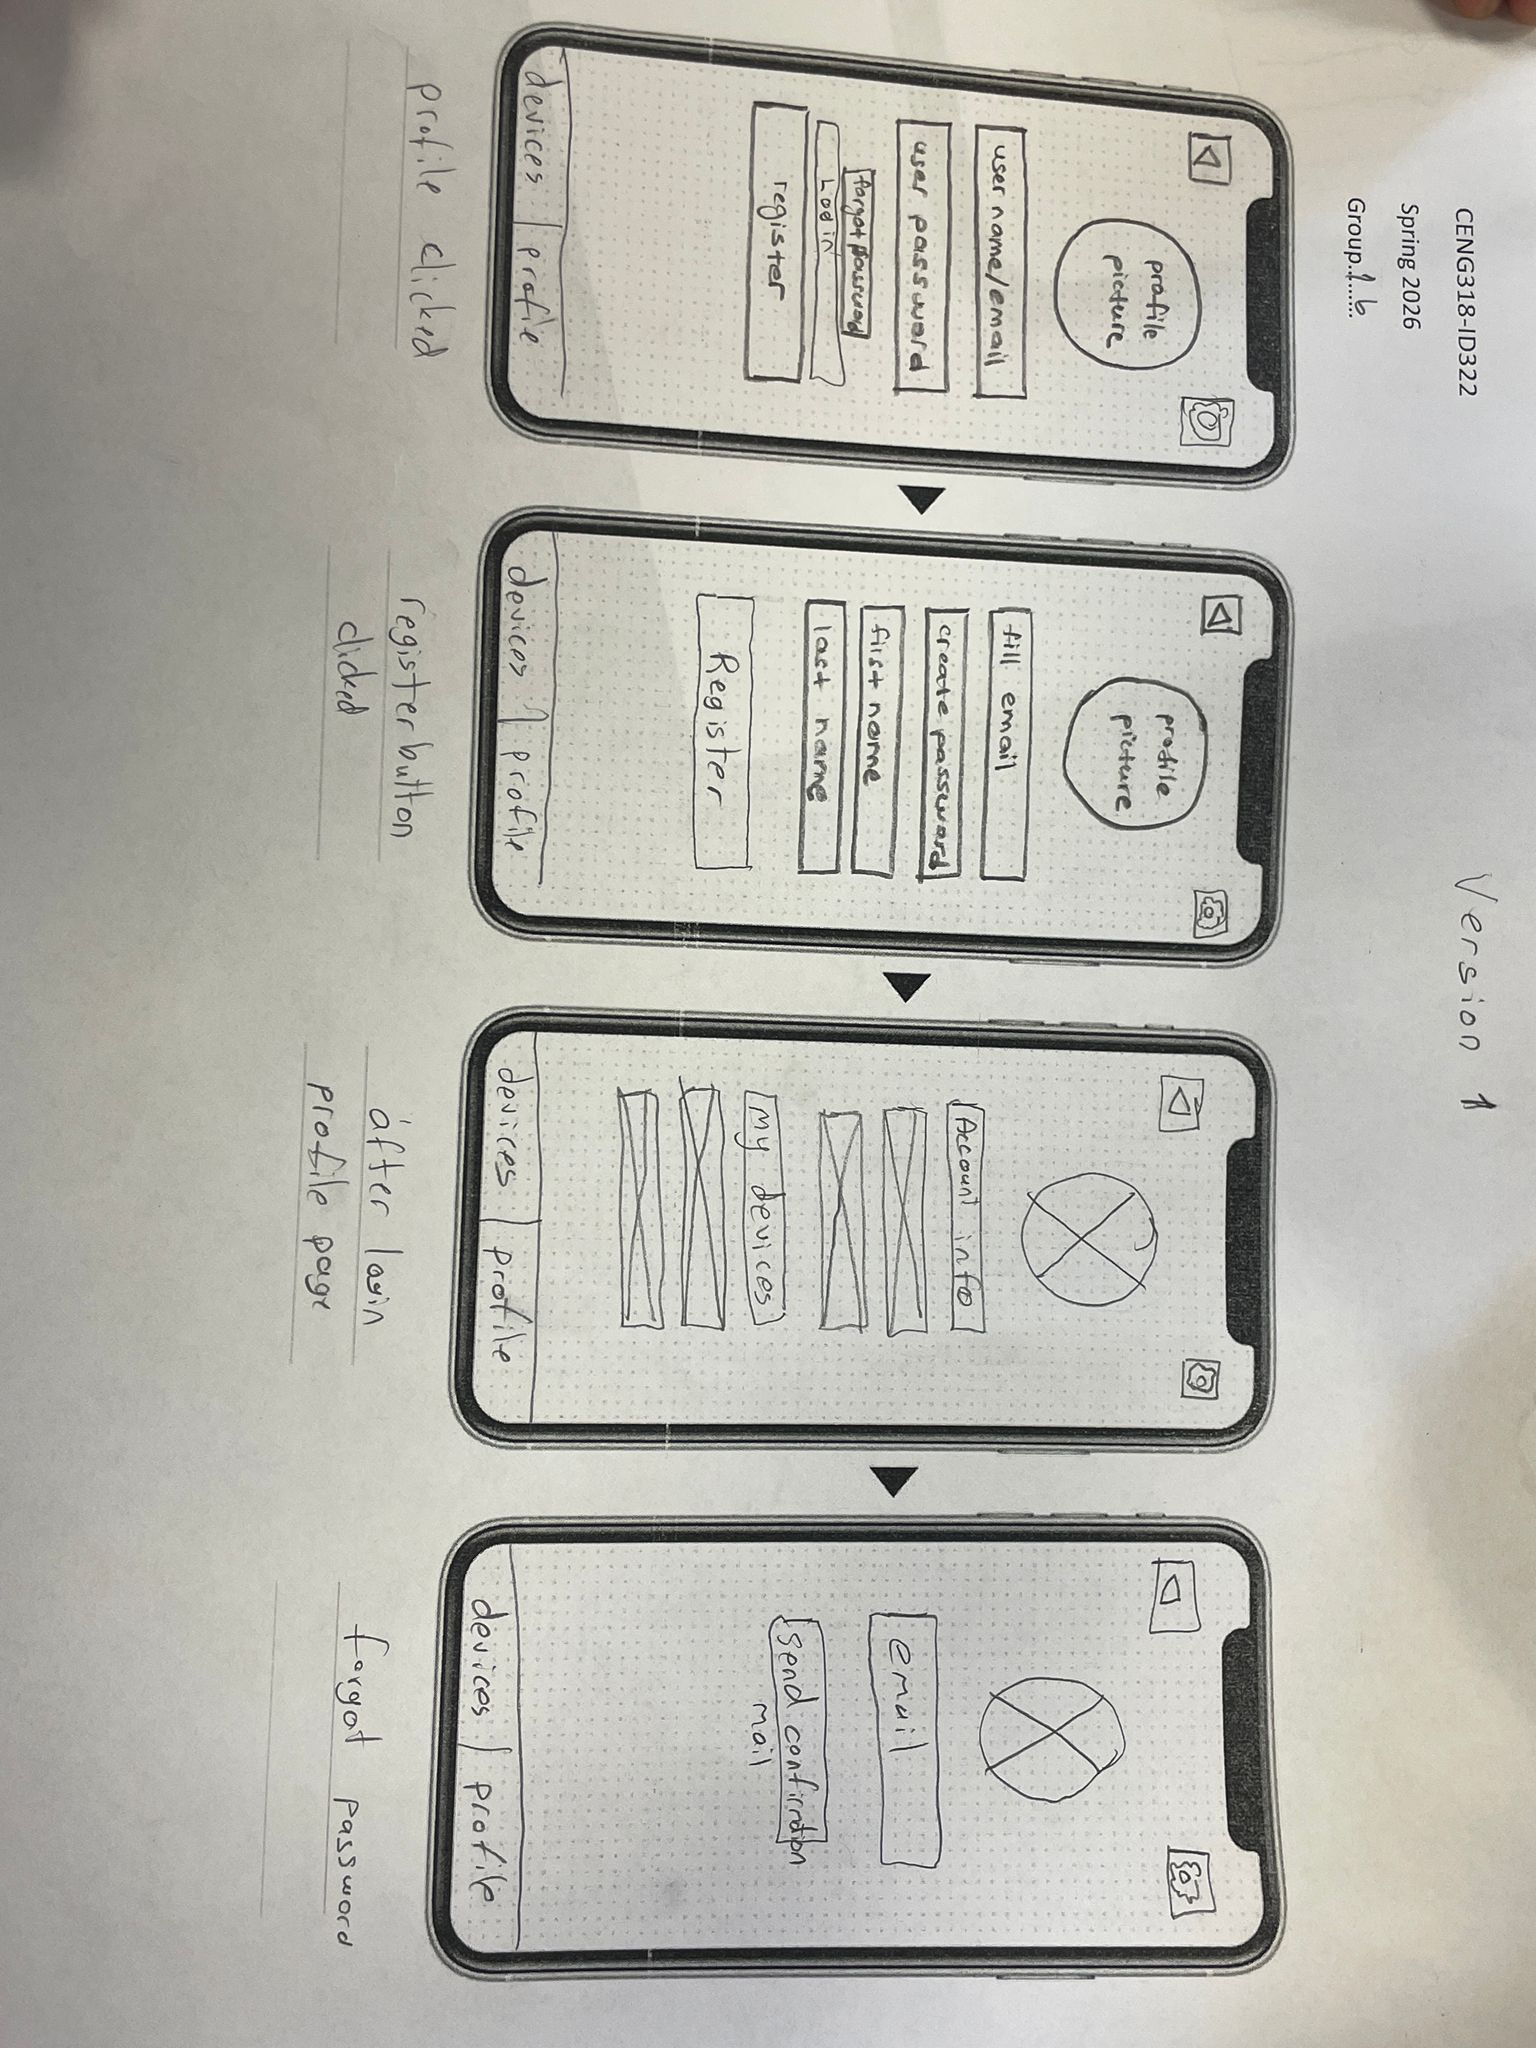
\includegraphics[width=0.82\textwidth]{flowsheets/flowsheet-auth-and-profile.jpeg}
  \caption{Four-frame profile/auth flowsheet: (1) Login $\to$ (2) Register $\to$
    (3) Profile after login $\to$ (4) Forgot Password.}
  \label{fig:v1-flow-auth}
\end{figure}

\subsection{Bluetooth Pairing Transition}

\begin{figure}[H]
  \centering
  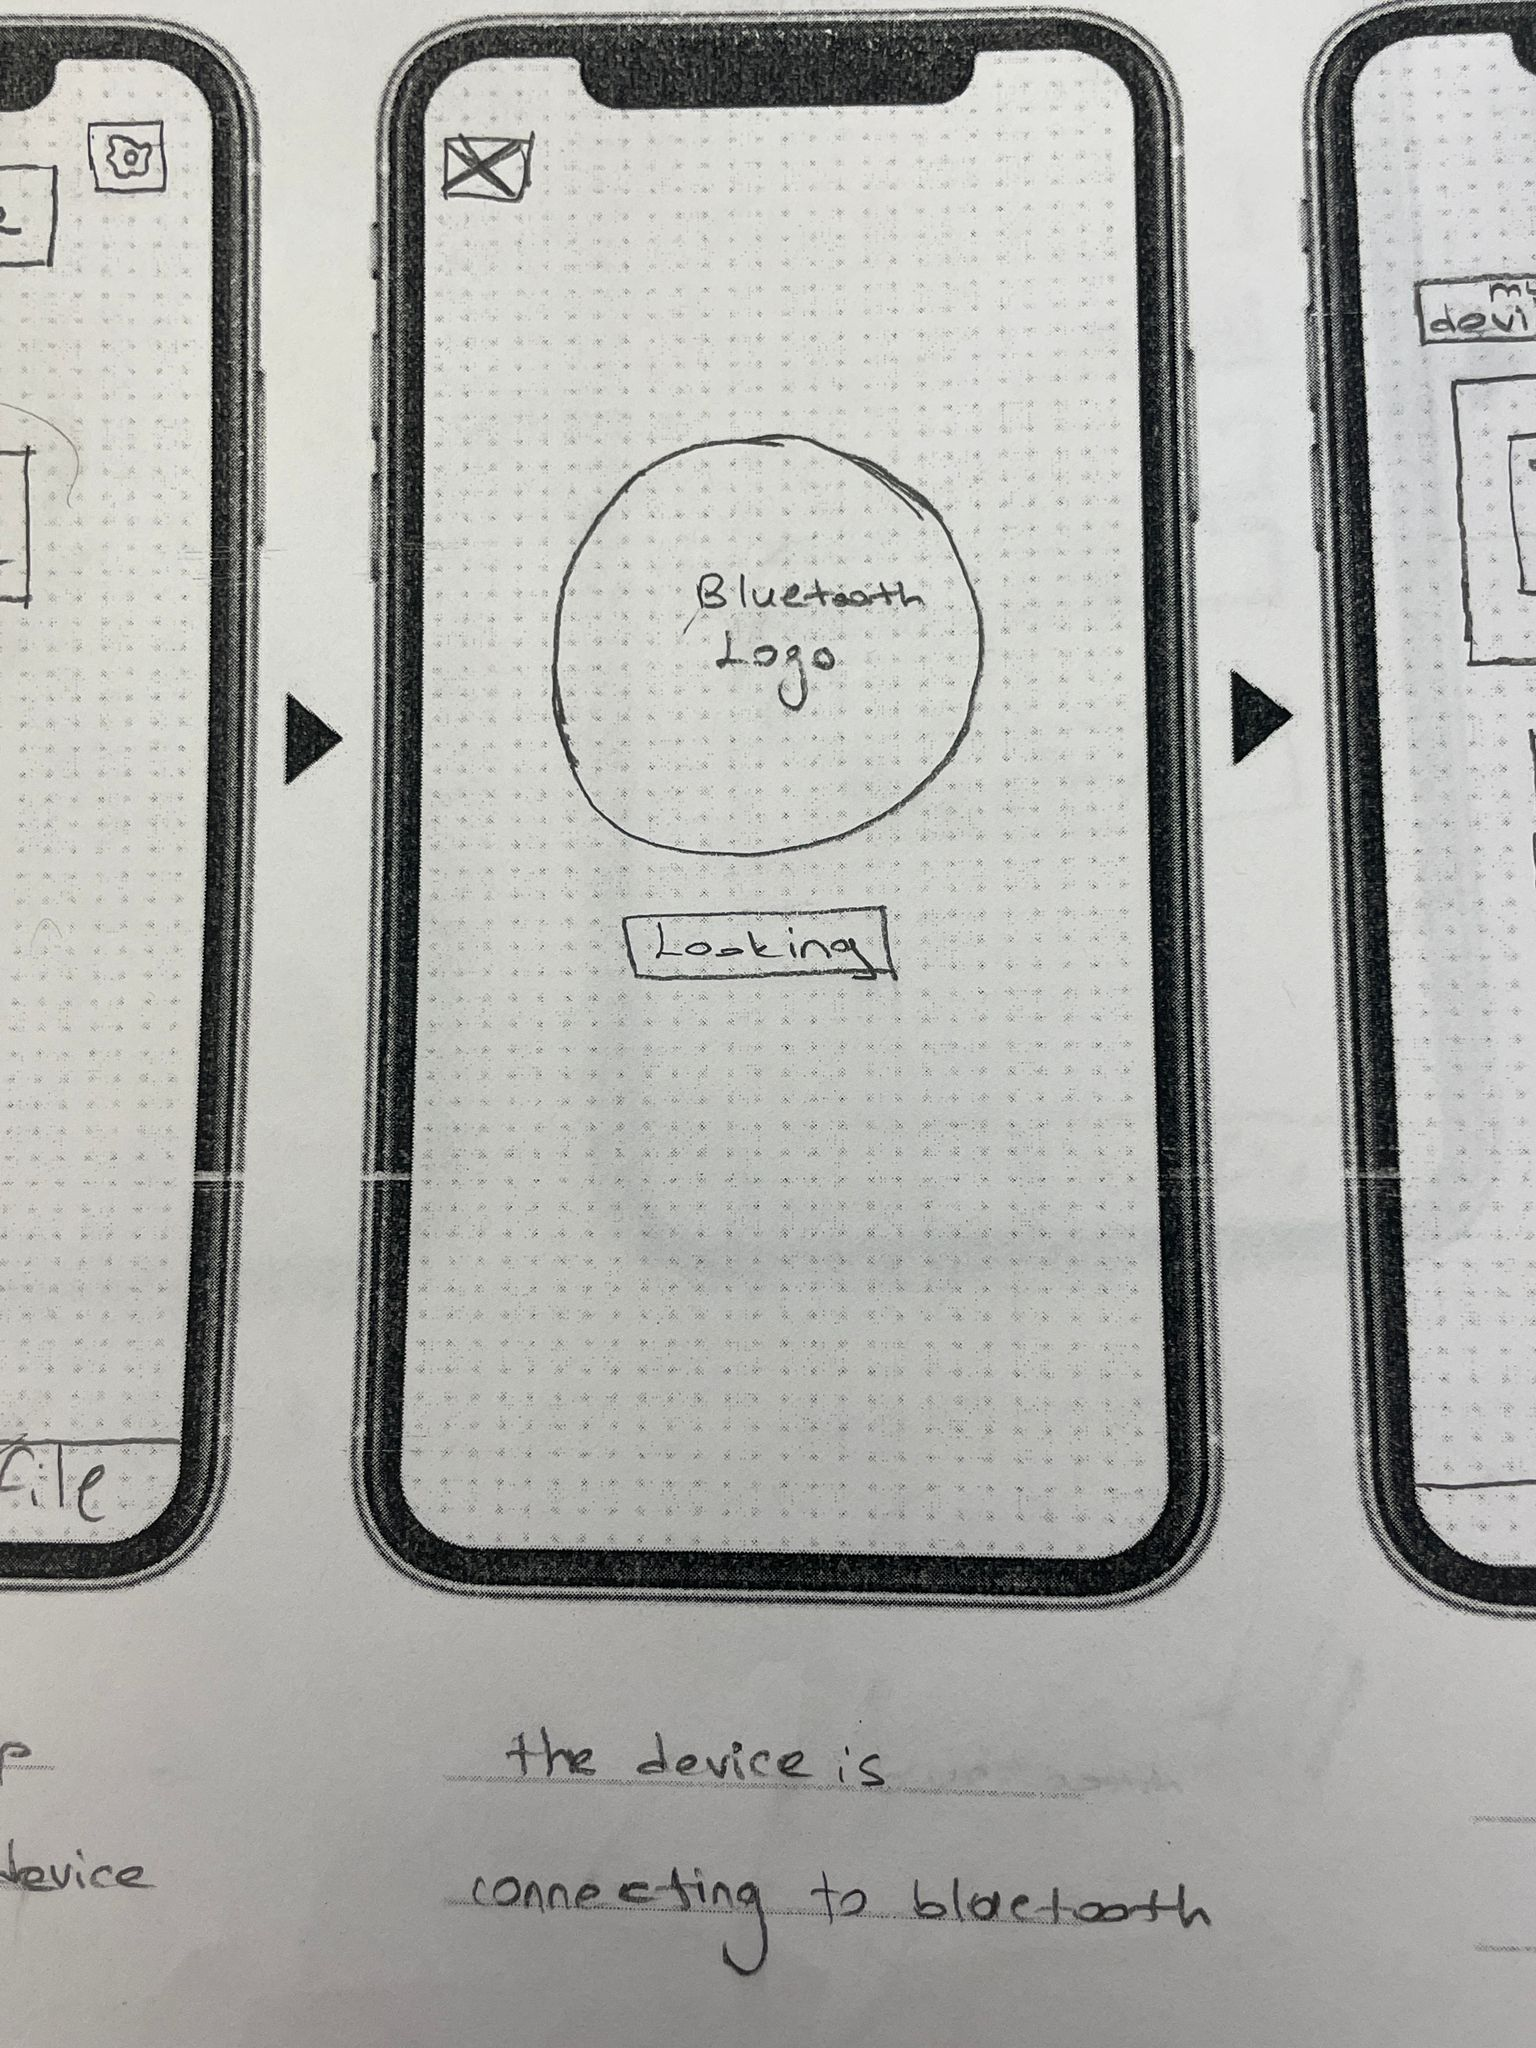
\includegraphics[width=0.82\textwidth]{flowsheets/flowsheet-bluetooth-pairing.jpeg}
  \caption{Pairing strip: Bluetooth ``looking'' screen between the previous screen
    and the My Devices list. Highlights the in-progress state.}
  \label{fig:v1-flow-bt}
\end{figure}

\subsection{Device Settings \& Power-Off Flow}

\begin{figure}[H]
  \centering
  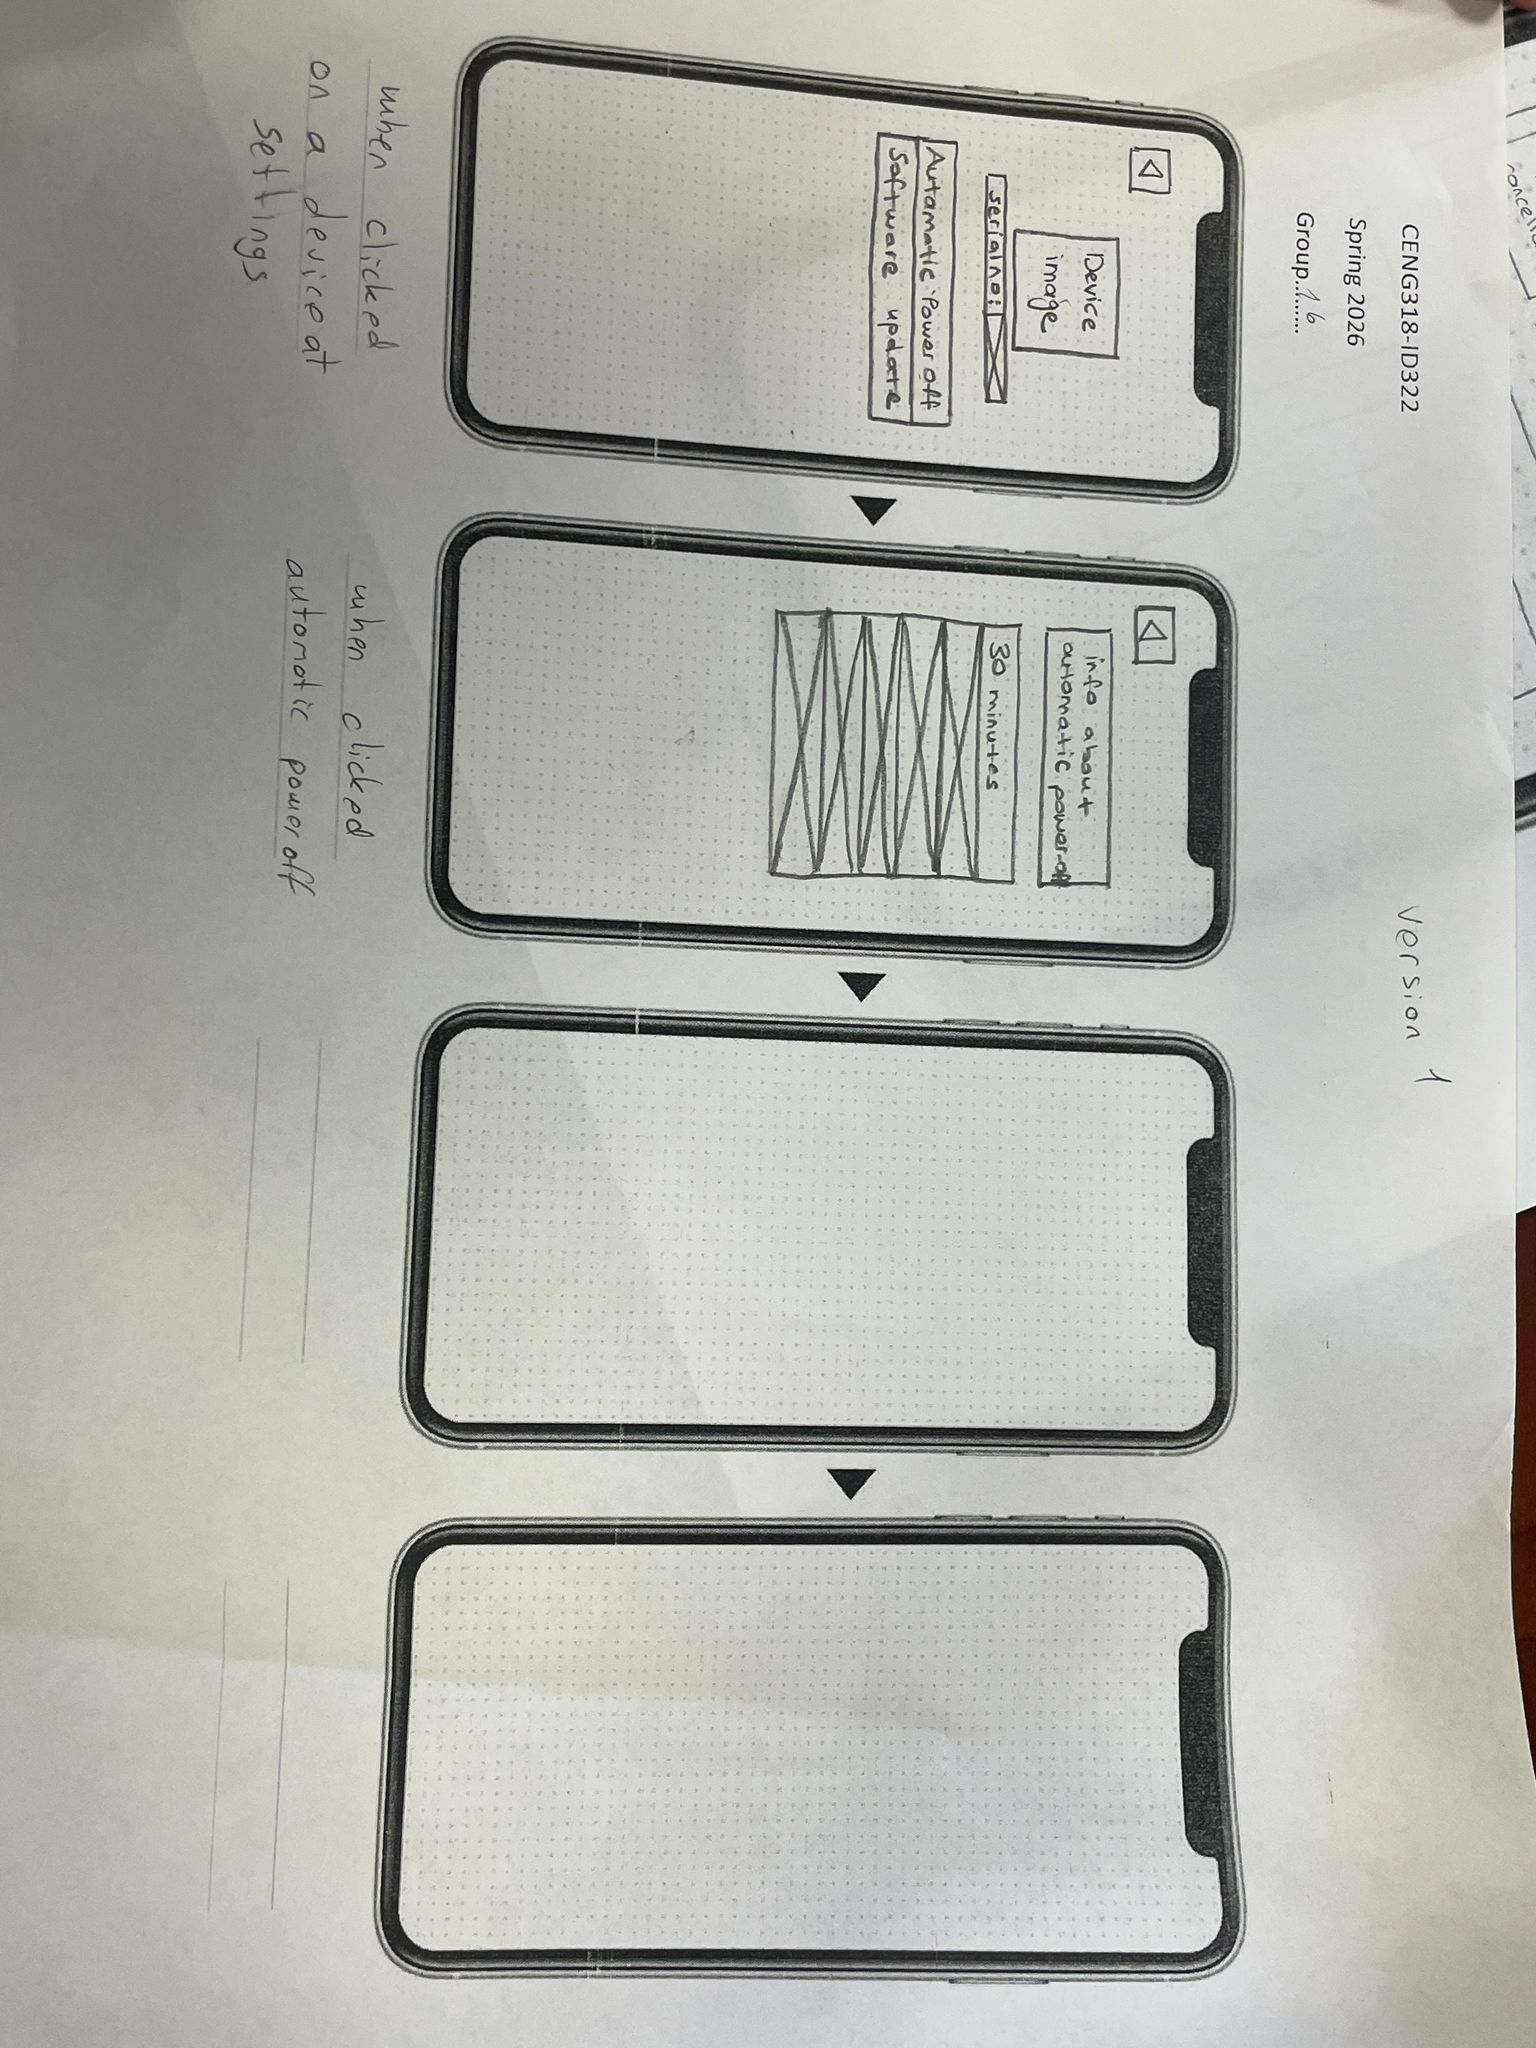
\includegraphics[width=0.82\textwidth]{flowsheets/flowsheet-device-settings-and-power-off.jpeg}
  \caption{Settings drill-down: Device Detail $\to$ Automatic Power-Off picker
    $\to$ placeholder frames for future steps.}
  \label{fig:v1-flow-settings}
\end{figure}

% ============================================================
\chapter{Design Rationale --- Version 1 to Version 2}
% ============================================================

This chapter explains what was learned from Version~1 and the specific decisions
that drove the changes in Version~2.

\section{Issue: Overcrowded Device Control Screen}

Version~1 combined the listening mode selector and a large multi-band equalizer on
a single device-control screen (Figure~\ref{fig:v1-device-eq}). In review, this
surface was too dense: users scanning for a quick mode switch had to visually
compete with equalizer sliders, and vice versa.

\begin{highlight}
  \textbf{Decision:} Split the combined screen into two dedicated tabs ---
  \textbf{Sound} (presets and EQ sliders) and \textbf{Noise} (listening mode
  selector) --- so each function occupies its own focused surface.
\end{highlight}

\section{Issue: Two-Tab Navigation Was Too Sparse}

The two-tab structure (Devices / Profile) meant that the most frequent audio
actions were buried behind a gear icon or a device card tap. Users had to follow
a non-obvious path to reach anything audio-related.

\begin{highlight}
  \textbf{Decision:} Expand to four tabs --- \textbf{Home}, \textbf{Sound},
  \textbf{Noise}, \textbf{Profile} --- so the two highest-frequency audio actions
  are always one tap away from any screen.
\end{highlight}

\section{Issue: No Volume Quick-Access}

Version~1 had no defined interaction for adjusting volume on the fly. Users expected
to change volume without navigating away from whatever screen they were on.

\begin{highlight}
  \textbf{Decision:} Add a \textbf{Volume overlay} --- an ephemeral modal capsule
  with a percentage readout --- that slides in over the current screen and dismisses
  by tapping outside. This keeps the user in context.
\end{highlight}

\section{Issue: No Usage Statistics Screen}

Version~1 had no way for users to see how much they had listened or whether they
were within safe listening levels. Feedback indicated this was expected.

\begin{highlight}
  \textbf{Decision:} Add a \textbf{Statistics} surface under the Sound tab, showing
  total listening time, a historical chart (day / week / month filters), and a safe
  listening indicator.
\end{highlight}

\section{Issue: Preset-Only Sound Was Inflexible}

Providing only preset buttons (Bass Boost, Balanced, Podcast) did not allow users
to fine-tune sound to their preference.

\begin{highlight}
  \textbf{Decision:} Add a \textbf{Custom} preset that unlocks Bass, Mid, and Treble
  sliders. A dedicated \textbf{Save} button commits the custom profile to avoid
  accidental changes.
\end{highlight}

\section{Issue: No Earbud Gesture Configuration}

Version~1 had no screen for assigning tap gestures (e.g.\ double-tap = Next Song)
to individual earbuds.

\begin{highlight}
  \textbf{Decision:} Add separate \textbf{Left bud} and \textbf{Right bud} screens
  under My Devices, each listing the assignable actions with a checkmark on the
  current selection.
\end{highlight}

% ============================================================
\chapter{Version 2 --- Hand-Drawn Digital \& Figma Wireframes}
% ============================================================

\section{Overview}

Version~2 introduced two parallel workstreams: \textbf{hand-drawn digital screens}
(drawn on a tablet) and \textbf{Figma wireframes}. Both adopt the four-tab navigation
established in the Version~1 review. Version~2 also added consolidated flow sheets
--- a nine-screen overview and a five-panel statistics/bud sheet --- to validate the
complete navigation hierarchy before moving to high-fidelity work.

% -------------------------------------------------------
\section{Hand-Drawn Digital Screens}
% -------------------------------------------------------

\subsection{Sound Tab --- Presets \& Sliders}

\begin{figure}[H]
  \centering
  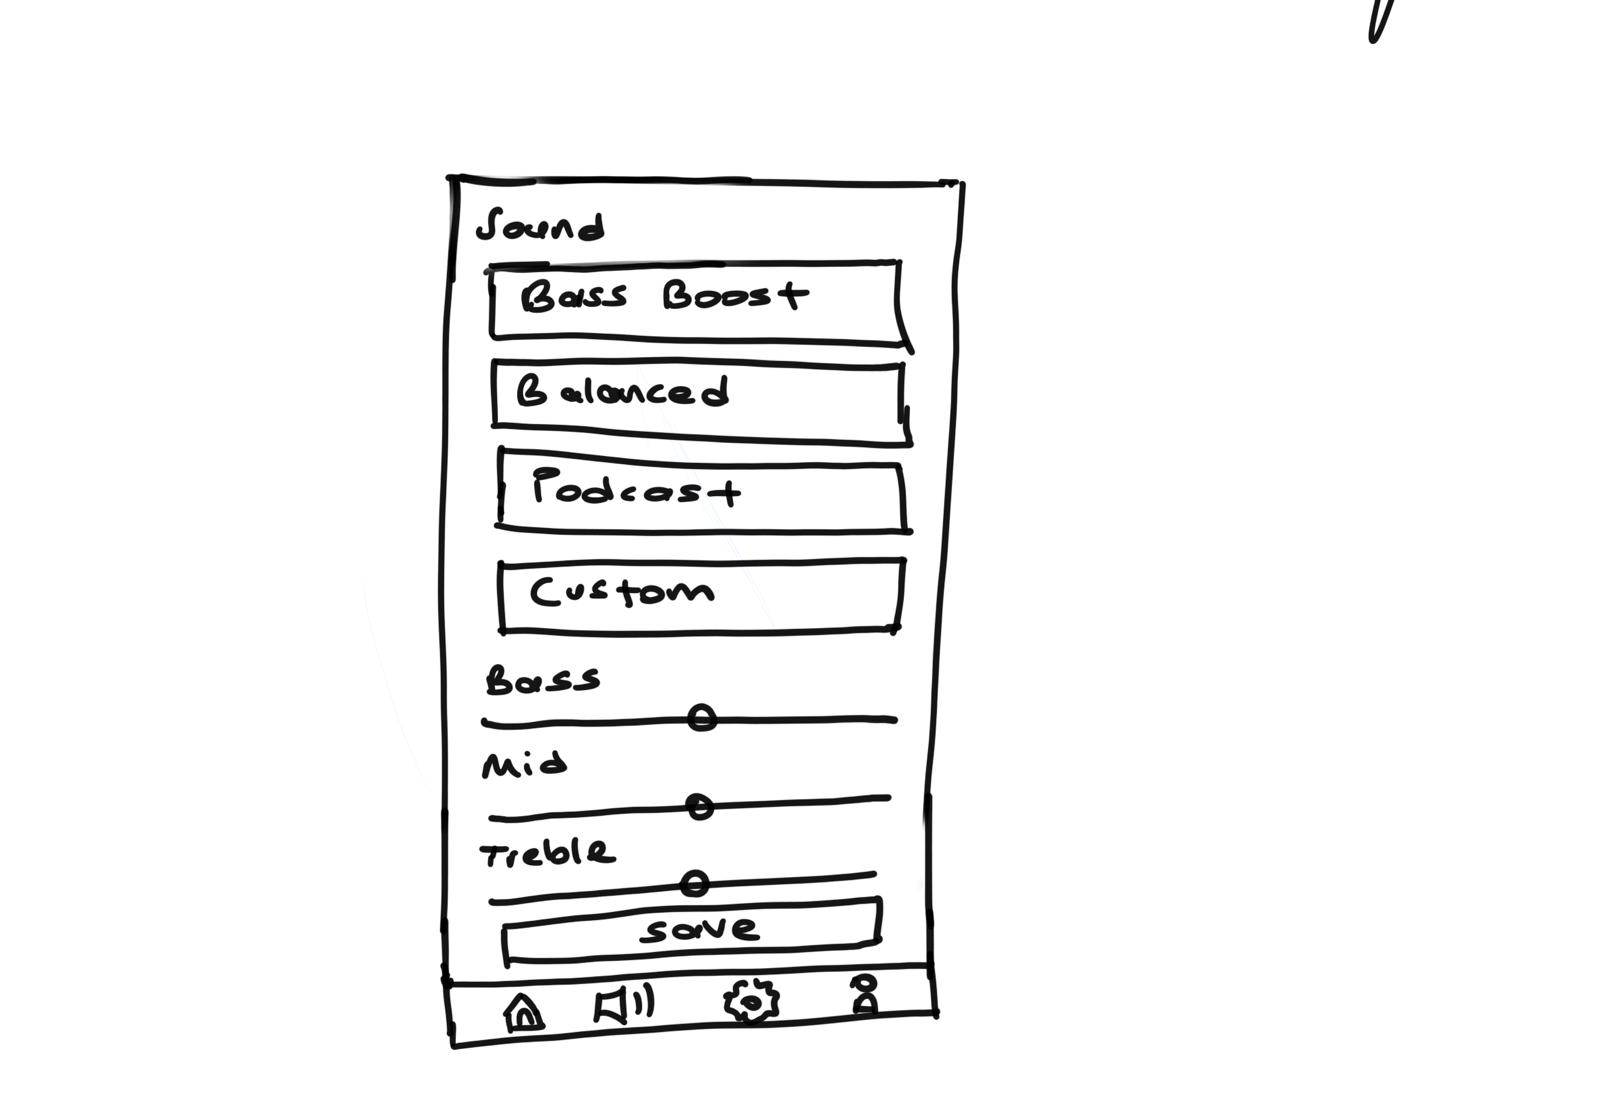
\includegraphics[width=0.80\textwidth]{hand-drawn/wireframe-sound-equalizer-presets-sliders.jpeg}
  \caption{Hand-drawn Sound screen. Four preset buttons (Bass Boost, Balanced,
    Podcast, Custom); Bass/Mid/Treble horizontal sliders; Save CTA below.
    Bottom nav: Home \textbar{} Sound (active) \textbar{} Settings \textbar{}
    Profile.}
  \label{fig:v2-hand-sound}
\end{figure}

\subsection{Volume Overlay}

\begin{figure}[H]
  \centering
  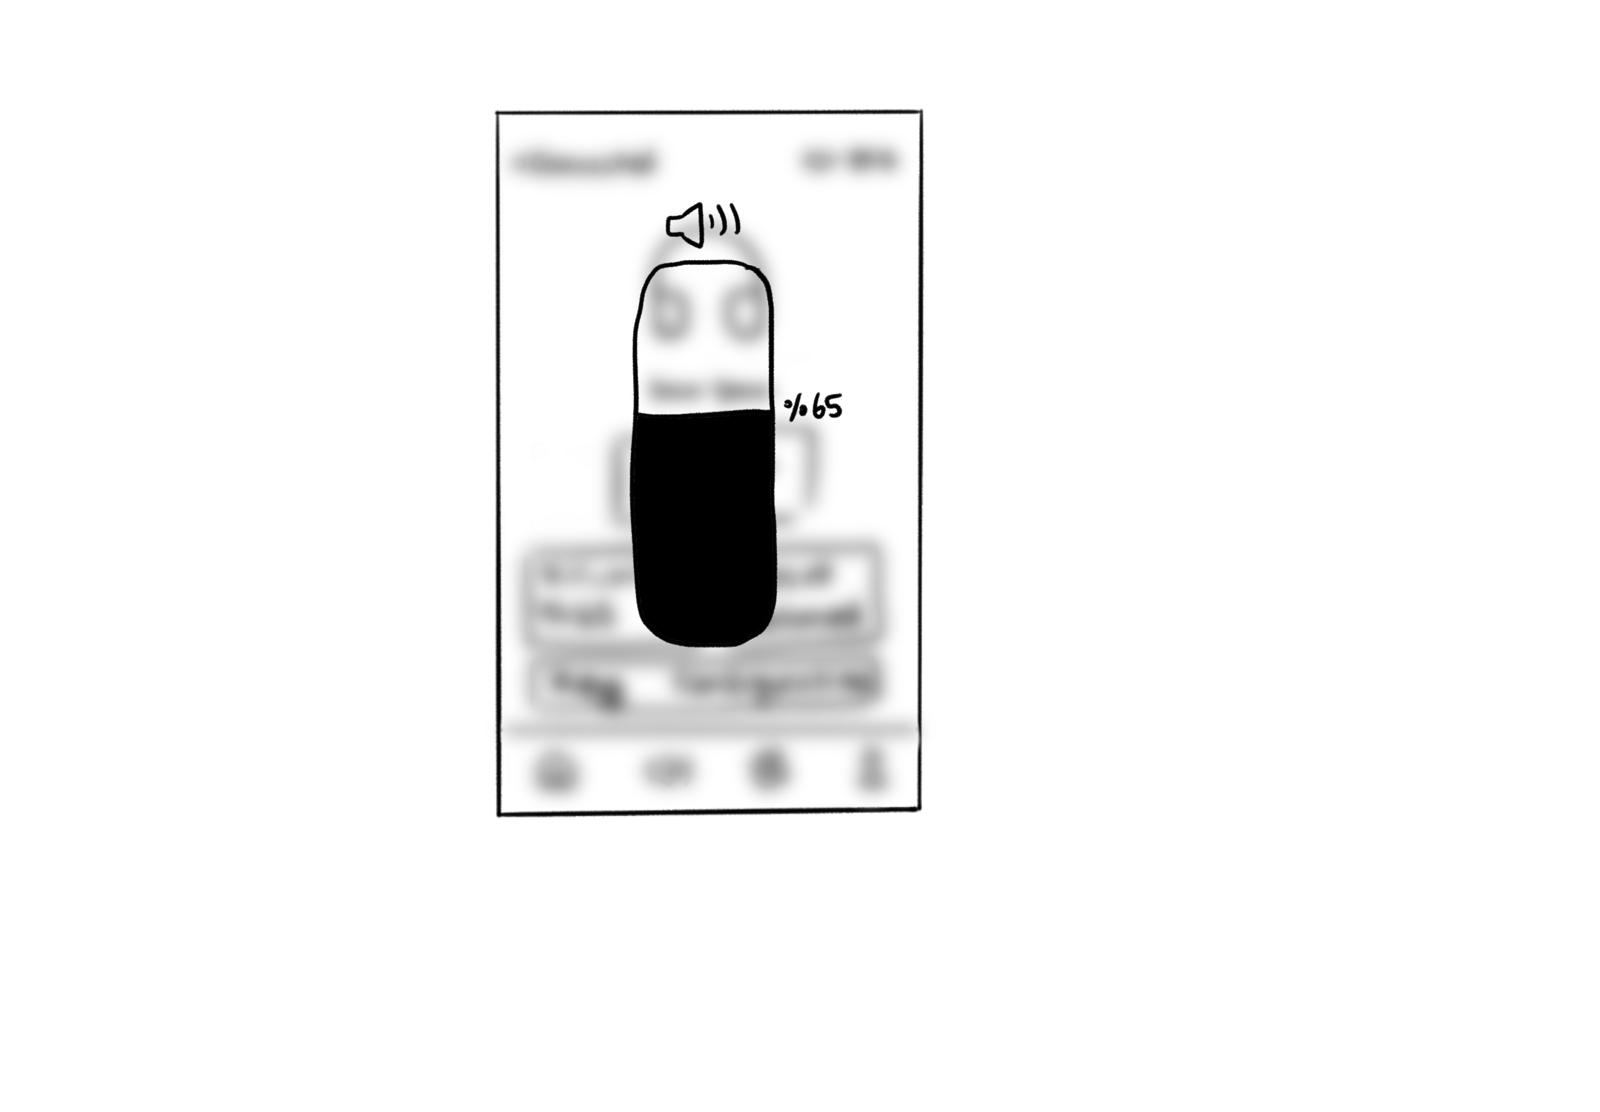
\includegraphics[width=0.80\textwidth]{hand-drawn/wireframe-volume-overlay-vertical.jpeg}
  \caption{Volume overlay: a modal vertical capsule placed over the blurred app
    chrome. The annotation ``\%65'' marks the current level. Tapping outside
    dismisses the overlay and returns to the previous screen.}
  \label{fig:v2-hand-volume}
\end{figure}

% -------------------------------------------------------
\section{Figma Digital Wireframes}
% -------------------------------------------------------

\subsection{Sound Tab --- Four Presets State}

\begin{figure}[H]
  \centering
  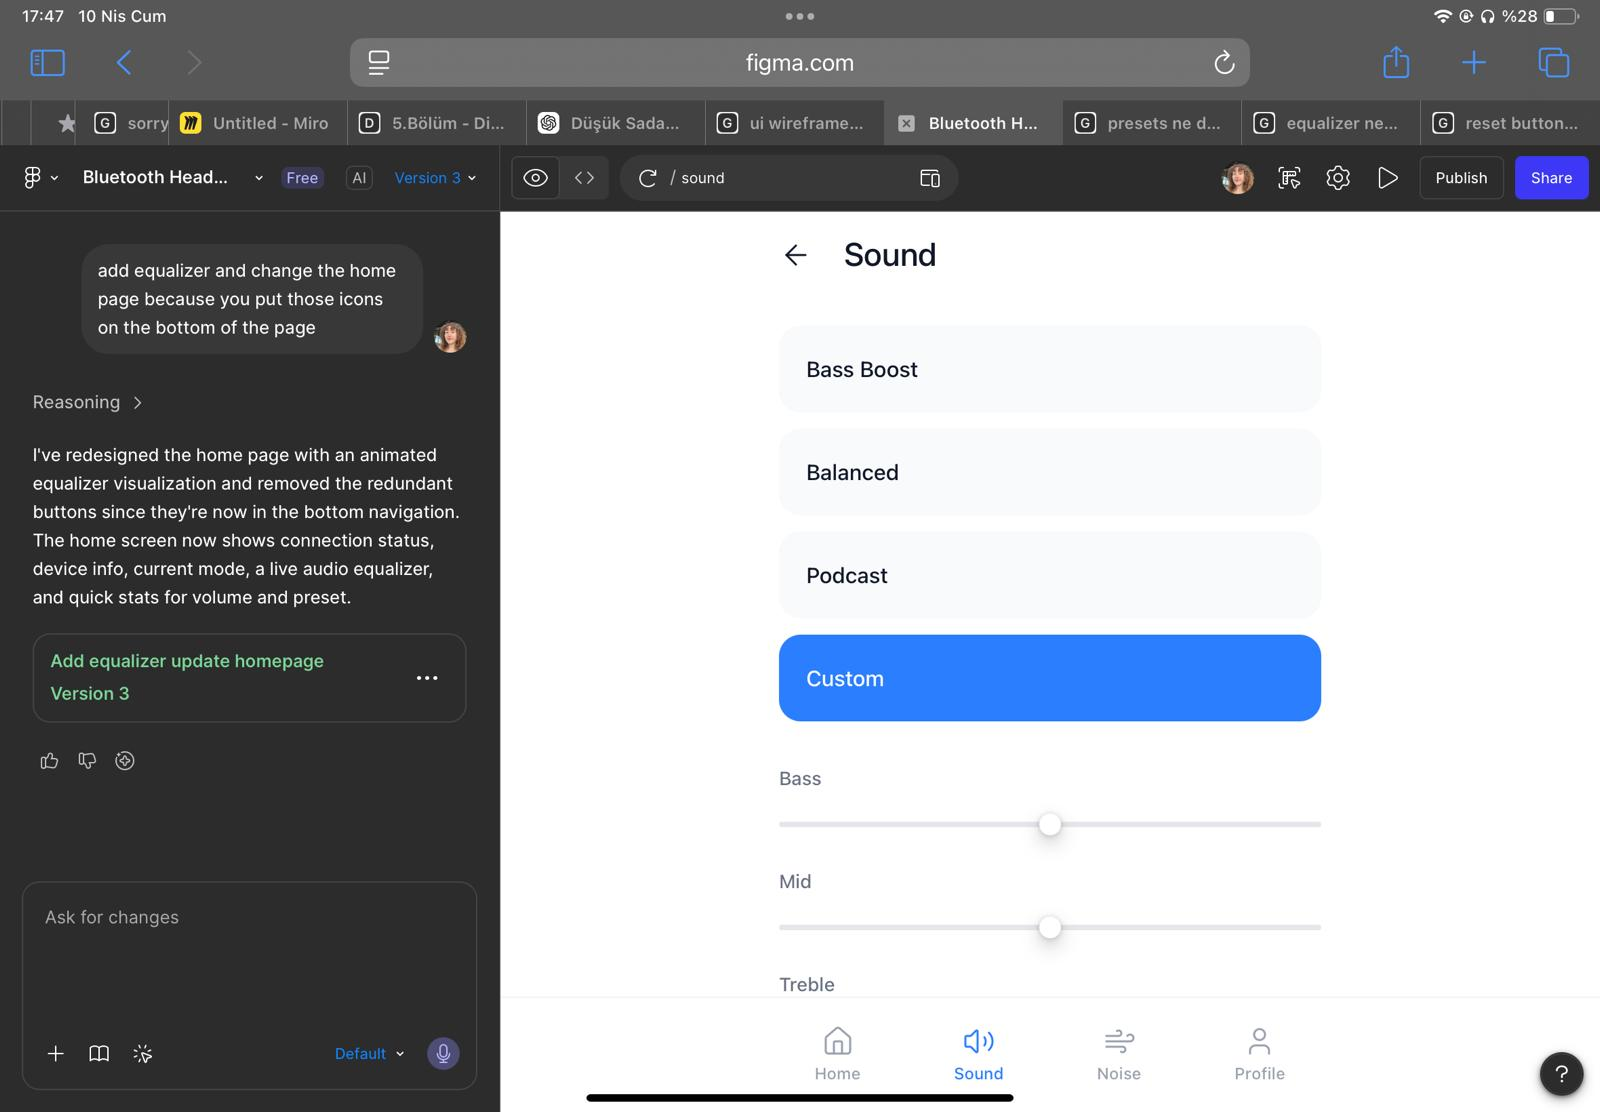
\includegraphics[angle=90, width=0.50\textwidth]{figma-v3/wireframe-sound-equalizer-four-presets.jpeg}
  \caption{Figma v3 --- Sound tab, preset selection. Pill buttons: Bass Boost,
    Balanced, Podcast, Custom (Custom active). Bass, Mid, Treble sliders below.
    Bottom nav: Home \textbar{} Sound (active) \textbar{} Noise \textbar{} Profile.}
  \label{fig:v2-figma-presets}
\end{figure}

\subsection{Sound Tab --- Custom Preset with Save}

\begin{figure}[H]
  \centering
  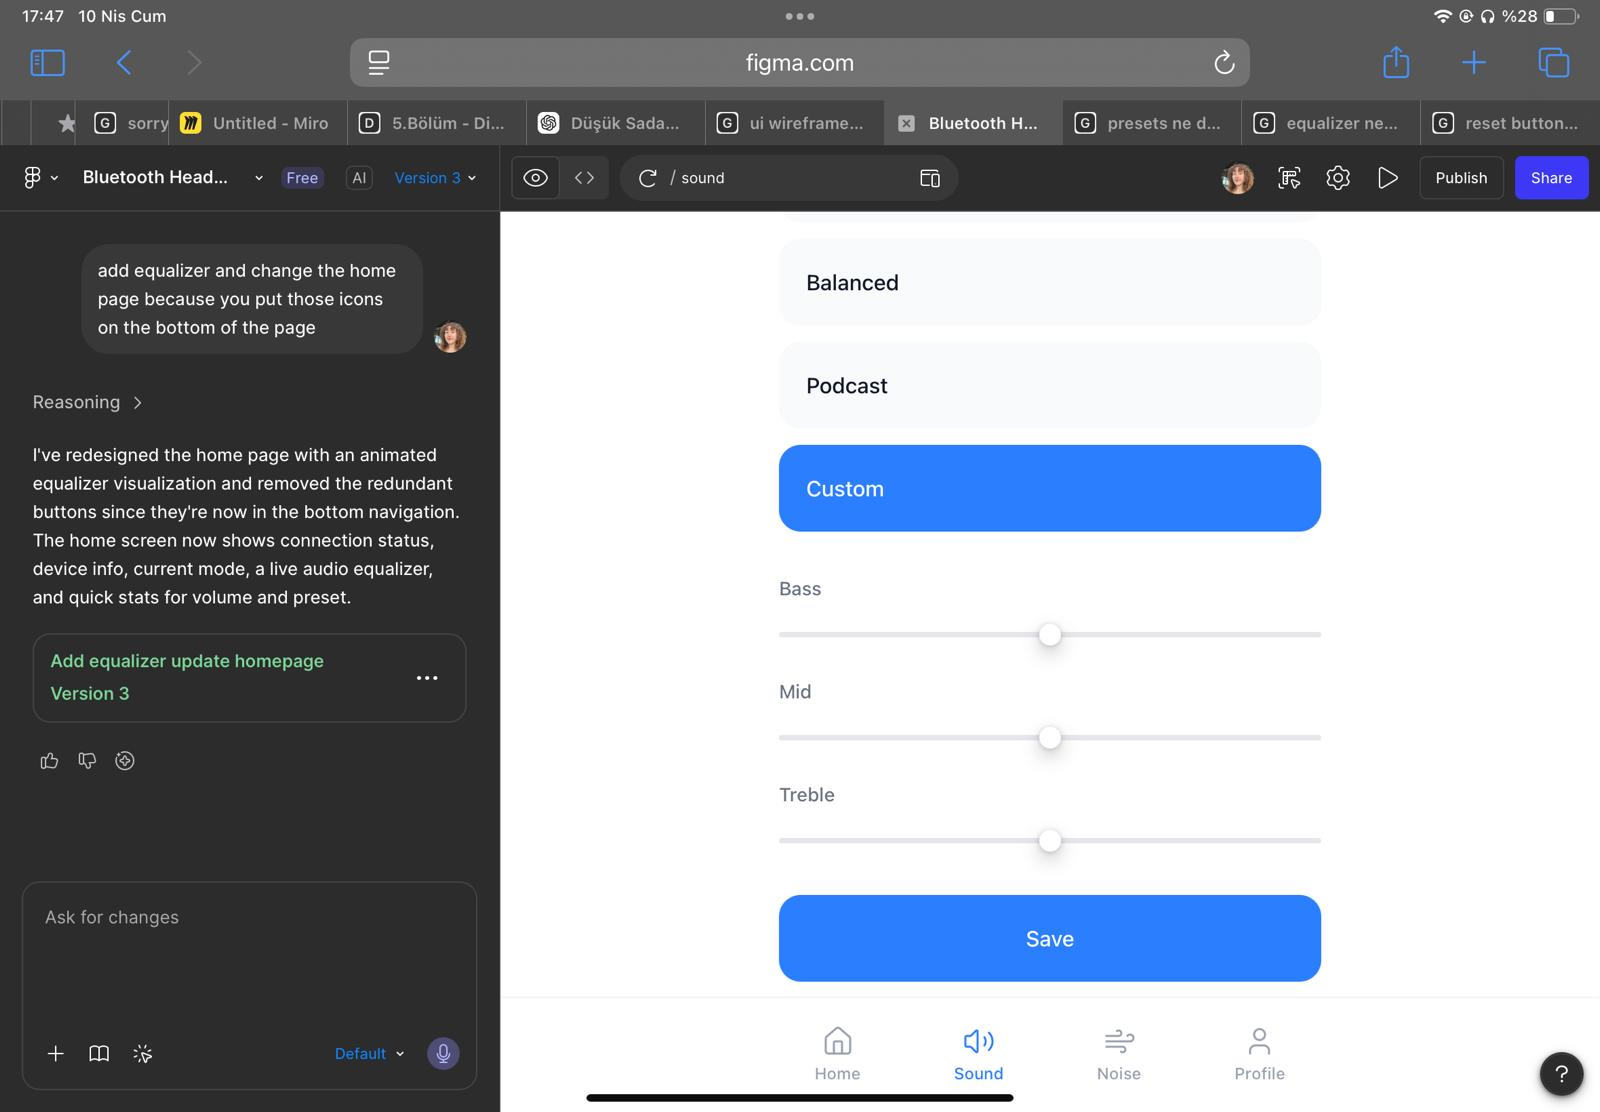
\includegraphics[angle=90, width=0.50\textwidth]{figma-v3/wireframe-sound-equalizer-custom-save.jpeg}
  \caption{Figma v3 --- Sound tab, Custom preset active with Save. A full-width
    blue \textbf{Save} button below the sliders commits the custom EQ profile.}
  \label{fig:v2-figma-save}
\end{figure}

The two Figma screens (Figures~\ref{fig:v2-figma-presets}
and~\ref{fig:v2-figma-save}) refine the hand-drawn version: the tab names are
finalised as Home / Sound / Noise / Profile (the hand-drawn version used Settings
instead of Noise as the third tab), and the Save action is visually prominent.

% -------------------------------------------------------
\section{Version 2 Flowsheets}
% -------------------------------------------------------

\subsection{Nine-Screen Consolidated Flow}

\begin{figure}[H]
  \centering
  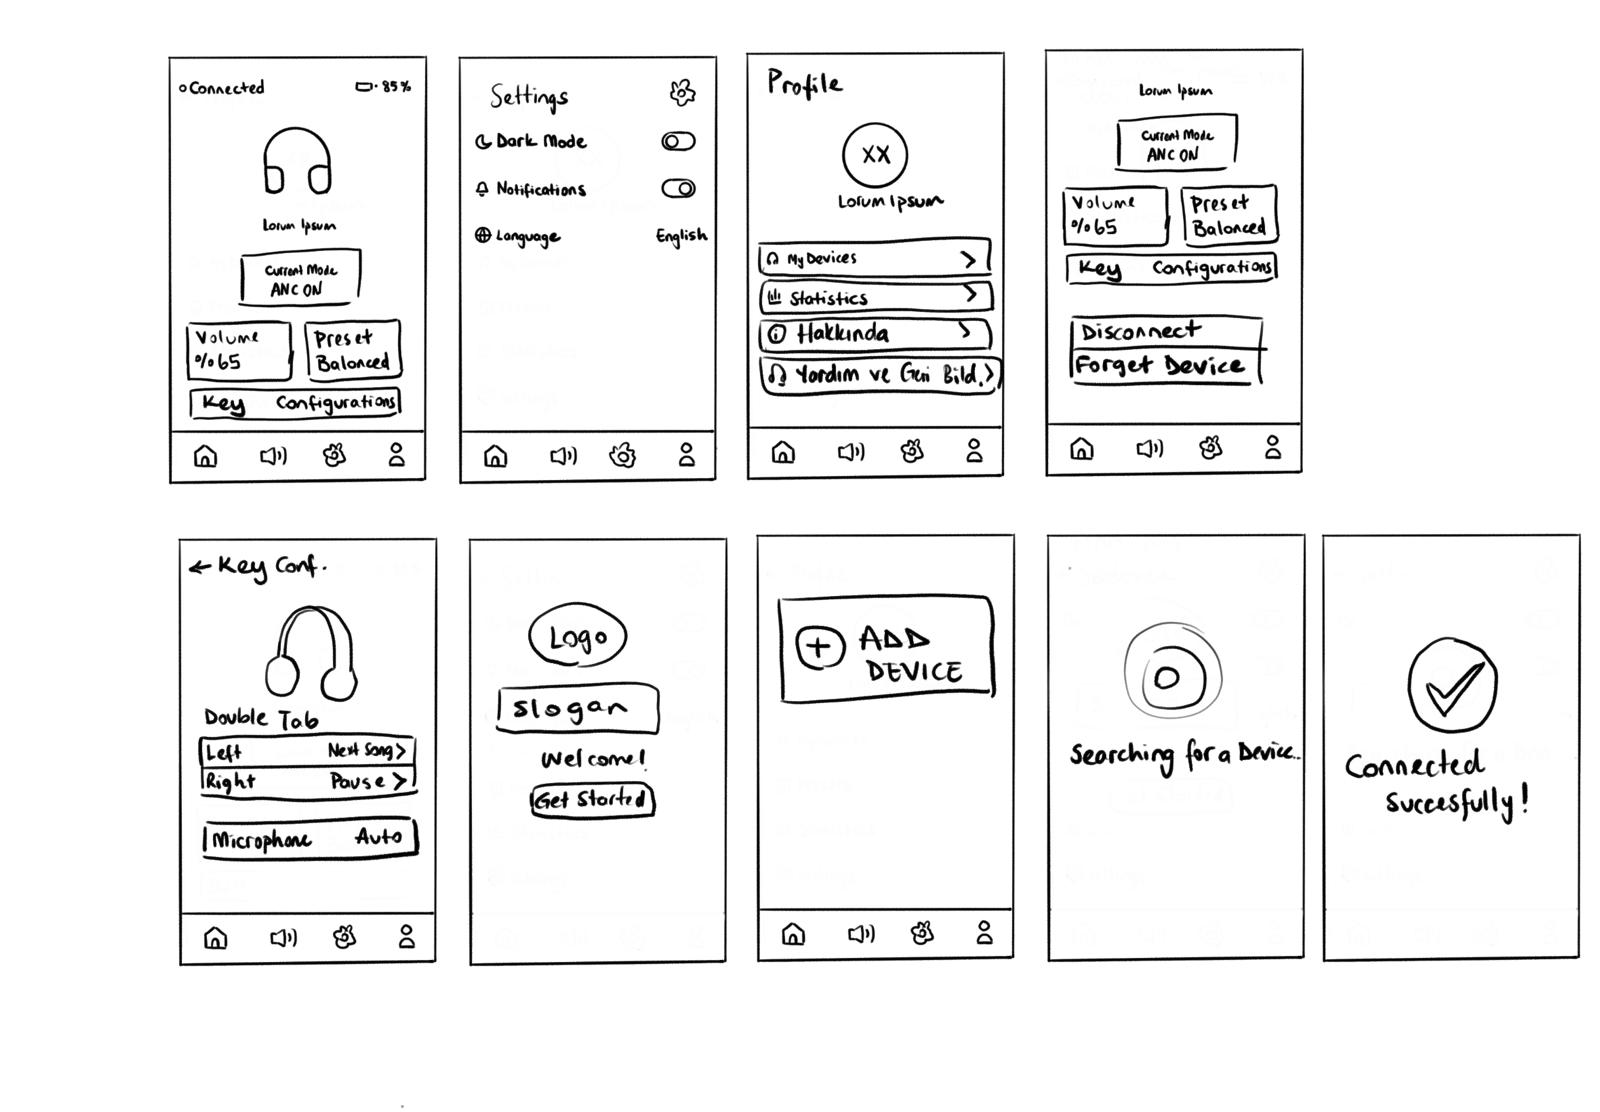
\includegraphics[angle=90, width=0.72\textwidth]{flowsheets/flowsheet-nine-screen-home-volume-settings-profile.jpeg}
  \caption{Nine-panel flow sheet covering the complete user journey: Splash $\to$
    Add Device $\to$ Searching $\to$ Connected $\to$ Home dashboard $\to$ Settings
    $\to$ Profile $\to$ Device Details $\to$ Key Configurations.}
  \label{fig:v2-nine-screen}
\end{figure}

\bigskip

\begin{center}
  \small
  \begin{tabular}{clp{8cm}}
    \toprule
    \textbf{\#} & \textbf{Screen} & \textbf{Key Content} \\
    \midrule
    1 & Splash / Landing   & Logo, slogan, ``Welcome!'', Get Started \\
    2 & Add Device         & Large ADD DEVICE (+), four-tab nav \\
    3 & Searching          & Radar motif, ``Searching for a Device\ldots'' \\
    4 & Connected          & Checkmark, ``Connected Successfully!'' \\
    5 & Home (Dashboard)   & Status, 85\% battery, ANC ON, Volume 65\%, Preset: Balanced,
                             Key Configurations button \\
    6 & Settings           & Dark Mode toggle, Notifications toggle, Language \\
    7 & Profile            & Avatar; My Devices, Statistics, About, Help \\
    8 & Device Details     & Dashboard summary + Disconnect / Forget Device \\
    9 & Key Configurations & Double-tap per earbud; Microphone: Auto \\
    \bottomrule
  \end{tabular}
\end{center}

\subsection{Five-Panel Statistics / Bud Controls Flow}

\begin{figure}[H]
  \centering
  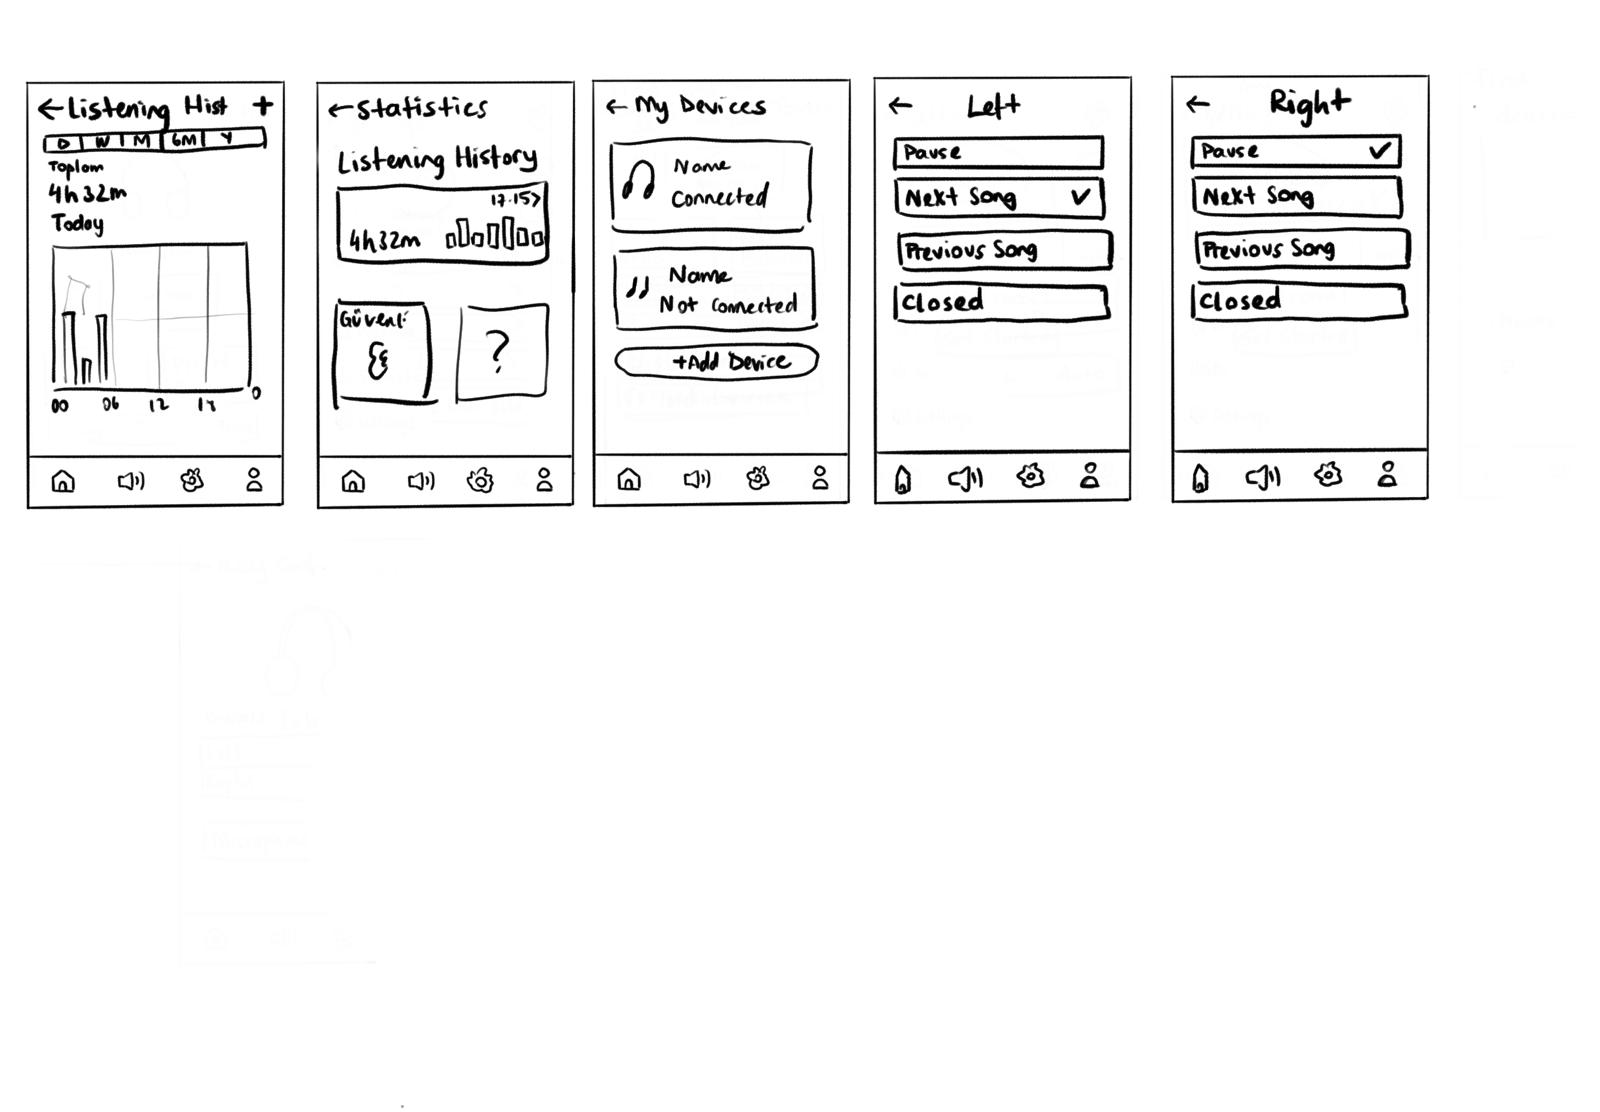
\includegraphics[angle=90, width=0.72\textwidth]{flowsheets/flowsheet-statistics-history-mydevices-bud-controls.jpeg}
  \caption{Five-panel flow: (1) Listening History chart, (2) Statistics card,
    (3) My Devices list, (4) Left bud gesture map, (5) Right bud gesture map.
    Bottom nav: Home / Audio / Settings / Profile.}
  \label{fig:v2-five-screen}
\end{figure}

\bigskip

\begin{center}
  \small
  \begin{tabular}{clp{8cm}}
    \toprule
    \textbf{\#} & \textbf{Screen} & \textbf{Key Content} \\
    \midrule
    1 & Listening History & D/W/M/6M/Y filters; Total 4h 32m; 24-hour bar chart \\
    2 & Statistics        & Listening History card (4h 32m); Safe listening indicator \\
    3 & My Devices        & Connected / Not Connected rows; + Add Device \\
    4 & Left Bud          & Pause / Next Song (selected) / Previous Song / Off \\
    5 & Right Bud         & Pause (selected) / Next Song / Previous Song / Off \\
    \bottomrule
  \end{tabular}
\end{center}

% ============================================================
\chapter{Design Reflection}
% ============================================================

\section{Key Design Decisions and Their Rationale}

\subsection{Home as the Central Hub}

Version~1 placed ``My Devices'' as the landing screen with no clear dashboard.
The Version~2 nine-screen sheet introduced a \textbf{Home dashboard} that shows
connection status, battery, current mode, volume, and preset at a glance, reducing
the number of taps needed for routine checks.

\subsection{Preset-First Sound Architecture}

Sound customisation is structured as \textit{presets first, sliders second}. Casual
users pick a preset in one tap; users who want manual control select Custom and
adjust the three-band EQ. The explicit Save button prevents accidental overwrite of
a saved profile.

\subsection{Noise Mode as a Separate Tab}

Merging noise mode into the Sound tab was considered and rejected. Switching noise
cancellation on and off is a high-frequency, context-driven action (entering a noisy
environment, making a call) that warrants its own tab rather than a secondary section
within Sound.

\subsection{Progressive Disclosure in Settings}

Settings uses a three-level drill-down: General Settings $\to$ Device Detail $\to$
Automatic Power-Off. Each level is entered only when the user explicitly navigates
deeper, reducing the risk of accidental changes to low-frequency preferences.

\section{Challenges}

\begin{enumerate}
  \item \textbf{Inconsistent tab labels across iterations.} Version~2 hand-drawn
    screens used Home / Sound / Settings / Profile, while Figma finalised Home /
    Sound / Noise / Profile. Resolving this required explicit agreement before
    high-fidelity work begins.
  \item \textbf{Density of the Version~1 device-control screen.} Deciding which
    controls belong on the main card vs.\ dedicated tabs took two review rounds.
  \item \textbf{Bluetooth state coverage.} Four distinct states (Empty, Searching,
    Connected Successfully, Dashboard) each required their own wireframe to avoid
    ambiguous transitions.
\end{enumerate}

\section{User Considerations}

\begin{itemize}
  \item \textbf{First-time users} see only Add Device on an empty home screen ---
    the next action is unambiguous.
  \item \textbf{Returning users} can change mode or preset in at most two taps
    from the Home dashboard.
  \item \textbf{System states} are shown explicitly (disconnected, searching,
    paired, connected) rather than toggling a single screen, reducing confusion.
\end{itemize}

% ============================================================
\chapter{Conclusion}
% ============================================================

Over two design versions the companion app UI evolved from a minimal two-tab paper
prototype into a structured four-tab interface with dedicated audio controls, usage
statistics, and earbud gesture configuration.

\begin{itemize}
  \item \textbf{Version 1} established the core screen vocabulary --- device list,
    profile/auth, settings --- using paper drawings and flowsheets to test
    transitions.
  \item \textbf{Version 2} addressed the gaps identified in review: the audio
    surface was split into Sound and Noise tabs, the combined device-control screen
    was decomposed, volume control became a quick overlay, and statistics + bud
    controls were added.
  \item All design decisions are driven by the principle that frequent actions
    (pairing, mode switch, preset select) must be reachable in at most one or two
    taps.
\end{itemize}

The resulting structure is ready to be taken into high-fidelity visual design and
implementation in the next project phase.

% ============================================================
\end{document}
% ============================================================
